\part{Produire et enrichir une édition numérique}

	%%%%%%%%%%%%%%% CHAPTER 4 %%%%%%%%%%%%%%%
	\chapter{De l'HTR à XML-TEI : mise en place d'une chaîne de transformation}
	\chaptermark{Mise en place d'une chaîne de transformation}
	
	Le déploiement d'une chaîne de traitement automatisée depuis les données océrisées vers le format XML-TEI (\textit{Text Encoding Initiative}) a fait l'objet de nombreux investissements de la part des laboratoires de recherches comme en témoigne les projets Artl@s, Katabase, \gls{dahn} ou encore le projet \gls{lectaurep}\footcite[Les travaux de Juliette Janès, de Lucie Rondeau du Noyer ou encore corbieresCatalogueAuFichier2020 sont particulièrement révélateur de velléités scientifiques.][]{rondeaudunoyerEncoderAutomatiquementCatalogues2019, corbieresCatalogueAuFichier2020, janesCataloguePapierAu2021}. L'objectif est d'assembler et structurer différentes briques de transformations afin de passer de l'image numérisée à une édition numérique native par le prisme du schéma \gls{tei}.
	
	L'intérêt pour l'application de ce format aux documents historiques résulte de sa grande polyvalence et adaptabilité, et ce peut importe l'origine ou la nature du document numérisé. Ce standard souhaite être le plus universel possible tout en rendant compte des singularités intrinsèques de chaque document et de son contexte d'origine. Lucas Terriel évoque ce schéma comme un \enquote{format pivot\footcite[p.~59]{terrielRepresenterEvaluerDonnees2020}} pour souligner les multiples exploitations possibles. 
	
	Toutefois, l'automatisation de données brutes vers ce format reste complexe, car elle fait face à un problème méthodologique et humaniste majeur. L'application d'un fichier \gls{tei} n'a de sens qu'en la joignant à une politique éditoriale ou scientifique et conjointement au document d'origine. La mise en place d'un protocole d'automatisation n'est valide qu'au sein d'un projet précis.
	
	À travers ce chapitre, nous cherchons à étudier les besoins, les réflexions et les défis auxquels s'est affronté ce projet d'édition des documents autour de l'Occupation de l'Araucanie. Ce projet s'est appuyé sur les précédentes expériences afin de concilier la retranscription des données aussi bien du point de vue quantitatif que qualitatif.
	
	\section{L’intérêt d’une édition numérique native}
	
	Avant de décrire plus en détail la mise en place de la chaîne de traitement éditorial, il convient de revenir sur les caractéristiques et les enjeux scientifiques de ce format pivot qu'est XML-TEI. Cette ébullition pour ce format dans le domaine des humanités numériques nécessite d'en considérer l'ensemble des aspects afin d'évaluer les ambitions scientifiques tout autant que les perspectives de valorisation autour de ce fonds.
	
	\subsection{L'édition numérique pour les humanités}
	
	De nombreuses préoccupations et interrogations sont apparues avec la prolifération des éditions électroniques à la fin des années 2000, notamment à la suite du mouvement \textit{Digital scholarship} britannique. La question du numérique remet pertinemment en cause l'ontologie du texte et sa textualité. Les projets d'ampleur tels que les éditions des \textit{Chroniques} de Jean Froissart\footnote{\textit{The Online Froissart}, version 1.4, éd. P. Ainsworth et G. Croenen, Sheffield, \url{https://www.hrionline.ac.uk/onlinefroissart/}.}, le roman \textit{Partonopeus de Blois}\footnote{\textit{Partonopeus de Blois}, Sheffield, \url{http://www.hrionline.ac.uk/partonopeus}.} ou les légendes arthuriennes\footnote{\textit{Queste del saint Graal}, éd. C. Marchello-Nizia et A. Lavrentiev, Lyon, Équipe BFM, publié en ligne par la Base de Français Médiéval, \url{http://portal.textometrie.org/bfm/?command=documentation&path=/GRAAL}.} ont été le support de développement de multiples textes autour de leurs apports et de leurs contraintes.
	
	Si l'hésitation entre le choix de l'orientation vers l'auteur ou le document demeure insoluble, de nombreux travaux linguistiques et philologiques considèrent que ces éditions numériques ne sont pas une altération, mais bien une solution pérenne pour les chercheurs. L'hypertexte devient un nouveau lieu de connaissances pour le scientifique et la constitution de son apparat critiques\footcite{duvalPourEditionsNumeriques2017}. La définition faite par la chercheuse humaniste Joana Casenave est particulièrement révélatrice des enjeux autour de l'édition électronique pour les humanités. Selon elle \enquote{L’édition numérique est [...] l’occasion d’un positionnement éditorial nouveau. Elle permet une diversification des informations présentées et une prise en compte de plus en plus forte des lecteurs au cours du travail philologique.\footcite{casenavePositionnementEditorialDans2019}}.
	
	La mise en place de ces projets a abondamment été commentée au gré des résultats des précédentes expériences éditoriales et scientifiques. Peter Robinson rappelle que la mise en place de ce type d'édition doit se faire dans le cadre d'une politique spécifique et s'appuyant sur cinq besoins : projets scientifiques particuliers, possession d'une transcription originale complète ou l'ouverture de ces transcriptions en données ouvertes, la valorisation et le changement de perception auprès du lecteur et enfin le projet d'établir des analyses quantitatives autour des textes\footnote{Robinson, Peter, \textit{What is a Critical Digital Edition?}, Variants. The Journal of the European Society for Textual Scholarship, 1, 2002. \textit{via} \footcite{vertongenQuEstceQu2022}}.
	
	Toutefois, Joana Casenave souhaite compléter cette définition autour de la notion de données ouvertes\footcite{casenavePositionnementEditorialDans2019}. La mise en place de ces éditions sous le format numérique permet d'augmenter les échanges autour de celle-ci. À la fois ouvert et en libre accès, il donne une nouvelle dimension au travail éditorial puisque celle-ci peut être axée sur des méthodes collaboratives, mais aussi sur la notion d'édition évolutive. La dimension socio-politique et scientifique des archives autour de l'Occupation de l'Araucanie a incité à mettre en place cette approche et expérience éditoriale.
	
	La construction d'un projet d'édition électronique native s'appuie aussi sur une volonté d'ouverture aux apports numériques au sein de la recherche fondamentale et la valorisation scientifique. Le développement des éditions numériques s'est fait en corrélation avec l'essor des humanités numériques en permettant l'exploration textuelle au travers de nouvelles méthodes scientifiques. La fouille de texte, la stylométrie, les analyses quantitatives ou la philologie numérique s'installent progressivement comme des méthodes heuristiques prépondérantes au sein des humanités\footcite{campsOuVaPhilologie2018}. Elles incarnent un rapport nouveau par rapport au texte et à la donnée avec un nouveau regard méthodologique introduisant la notion de reproductibilité\footcite{campsOuVaPhilologie2018}. Ces données ouvertes offrent de même la possibilité de développer des outils numériques d'analyses, autant que la valorisation du corpus.
	
	\subsection{\texttt{XML-TEI} : retour sur un format pivot}
	
	Avec la croissance des projets d'éditions numériques, le format XML-TEI s'est imposée comme un standard pour le développement de ce type de projet. La \gls{tei} est fondée sur la structuration de données \gls{xml} et une syntaxe précise permettant de définir et contraindre l'ensemble des éléments utilisés.
	
	En réalité, la \gls{tei} désigne initialement une communauté scientifique qui a ensuite donné son nom à cet encodage. La communauté académique a été fondée en 1987 afin de répondre aux nouveaux défis numériques, en proposant une première grammaire sous la forme d'une \gls{DTD} pour le format SGML (\textit{Standard Generalized Markup Language}), puis à son langage descendant \gls{xml}. Les objectifs de cet encodage sont de faciliter le traitement et l'échange des données textuelles, en préférant des solutions générales et modulaires. Cette initiative s'inscrit dans une volonté de proposer un format de données conservant le sens informationnels et contextuels tout en affichant une indépendance claire avec les logiciels propriétaires \footcite[Lou Burnard, \enquote{Introduction} \textit{in}][]{burnardQuEstceQue2015}.
	
	L'association a depuis considérablement multiplié et enrichi son encodage depuis sa création, multipliant par cinq le nombre de balises disponibles. Ainsi, Jean-Baptiste Camps parle d'une \enquote{communauté de pratiques\footcite{campsTEICommunautePratiques2017}} pour évoquer le rôle de cette communauté et de cet encodage. La souplesse et l'accessibilité de ce standard en font des qualités indéniables puisqu'elles permettent aux différents projets de pouvoir l'adapter à leurs besoins et tout en conservant une certaine interopérabilité. Ces nombreuses qualités et sa constante amélioration ont été permises grâce à  une communauté active qui en a fait un format pivot majeur pour les humanités numériques. Ce format est aussi essentiel pour le lecteur car il offre une lecture accessible mais aussi la possibilité de déployer des outils numériques annexes. Le centre \gls{acab} a donc souhaité s'ouvrir et répondre à ces nouveaux enjeux numériques avec une expérimentation autour de ces archives en proposant des données ouvertes et exploitables, mais aussi valoriser les données contenues par ces documents. 
	
	\subsection{Les outils numériques de valorisation}
	
	Avec l'ébullition de l'encodage \gls{tei} au sein des humanités numériques, une pluralité d'outils a accompagné la mise en place d'éditions nativement numériques. Afin de préparer ce projet d'édition et de valorisation des sources du conflit entre l'État chilien et les tributs Mapuches, trois applications ont été étudiées. Afin d'en déterminer les avantages et les inconvénients. Par manque de temps, le développement n'a pu être mis en application restant pour le moment à l'état de prospection.
	
	La première étude fut centrée sur l'utilisation d'un \gls{CMS} très connue au sein des institutions archivistiques : la plateforme Omeka. Elle permet de mettre en place rapidement et aisément une application dédiée à l'exploration et la visualisation des collections patrimoniales, ainsi qu'à leurs notices associées. Omeka possède une architecture minimaliste fondé sur le système LAMP (Linux Apache, MySQL, PHP) permettant d'être facilement exploitable ainsi que d'être sous licence libre et gratuite\footnote{\textit{OMEKA}, url: \url{https://omeka.org/about/project/}, consulté le 19/08/2022.}. Néanmoins, le nombre de possibilités permis par ce \gls{CMS} reste très limité de par sa structure volontairement rigide et simpliste. Ces caractéristiques ne permettent pas une exploitation exhaustive des données transcrites et n'offre qu'une très faible modularité\footnote{Ces problèmes ont été amplement commentés par Cécile Boulaire et Romeo Carabelli, \enquote{Du digital naive au bricoleur numérique : les images et le logiciel Omeka}, \textit{in} \cite{cavalieExperimenterHumanitesNumeriques2018}}.
	
	La seconde solution logicielle a été développée par la société internationale à but non lucratif \textit{e-editiones} sous le nom de \texttt{TEI Publisher}\footcite{TEIPublisher2022}. Cette application \textit{open-source} s'appuie sur \texttt{exist-db} qui est un système de gestion de base de données \gls{xml}. \texttt{TEI Publisher} offre une interface extrêmement complète avec la présence de nombreux modules très intéressants dont des fonctions de recherche plein texte ou à filtres, un système de pagination, la reconnaissance d'entités nommées, géolocalisation ou encore la compatibilité avec l'\gls{API} IIIF (\textit{International Image Interoperability Framework}). À partir de ces expérimentations, Hugo Scheitauer estime que cette plateforme offre une excellente solution moyen-terme pour la valorisation des corpus \gls{tei}\footcite[p.~139-143]{scheithauerReconnaissanceEntitesNommees2021}. La transformation \gls{xml} vers le langage web HTML s'effectue selon les règles définies au sein de l'\gls{ODD} accompagnant le corpus \gls{tei}. \texttt{TEI publisher} fournit ainsi une application extrêmement complète et à moindre coût technique et financier pour les institutions patrimoniales et scientifiques.
	
	Enfin, les prémices d'une application web ont été élaborées au sein de centre afin de dessiner les fonctionnalités nécessaires à la valorisation et l'exploration scientifique du corpus océrisé. Le développement d'une telle application permettrait \textit{de facto} d'établir et d'étoffer des fonctionnalités propres à l'exploration des données éditées. Toutefois, elle nécessite une maîtrise avancée de \textit{framework} web et de modules adaptés\footnote{Les frameworks \texttt{Flask} ou \texttt{Django} paraissent les plus aptes à ce type de projet puisque de nombreux modules complémentaires comme \texttt{Lxml} ou \texttt{folium} leurs sont compatibles.}. L'idée initiale est de centrer le projet auprès de la richesse des entités géographiques présentes au sein des différentes sources, en établissant une carte dynamique et des fonctionnalités de recherche à filtre permettant de retracer l'évolution narrative de la correspondance. Les travaux de Ludovic Moncla sont particulièrement éclairants sur l'automatisation des dynamiques spatiales à partir de la \gls{ren}\footcite{monclaAutomaticExtractionMethod2018}. Le projet à long terme souhaiterait développer cette contextualisation des dynamiques spatiales et de la géomatique en s'appuyant sur le georéférencement d'une carte historique du Chili.
	
	\section{XML-TEI et les archives océrisées du conflit Mapuche}
	
	Au regard de ces observations préliminaires, il doit être évoquer la méthodologie employée afin de transformer les fichiers \gls{alto} vers le format XMl-TEI. La mise en place d'un script python a nécessité un ensemble de réflexions sur la flexibilité de la transformation des transcriptions en fonction de la typologie du document et du schéma édité. Nous nous concentrons ensuite sur la validation du schéma et la documentation associée.
	
	\subsection{Convertir les données océrisées au format TEI} 
	
	Comme nous l'avons vu, de nombreux projets se sont appliqués à transformer les données \gls{alto} vers un schéma \gls{tei} préalablement défini. Selon les différentes méthodologies employées, la chaîne de traitement a été développé sur la base du langage python, et plus particulièrement la librairie \texttt{Lxml} , ou XSLT spécialisée dans la transformation \gls{xml}.
	
	Nous avons finalement pris le parti de nous appuyer sur le langage python en raison de ses performances, d'une communauté très active permettant de faciliter la maintenance et l'amélioration de l'application. De ce fait, nous avons repris la structure du \gls{cli} \texttt{Alto2tei} développée par Kelly Christensen\footcite{christensenAlto2tei2022}. Ce script a été développé dans le cadre du projet Gallic(opora) au cours de l'année 2022 dans le but de transformer les documents numérisés, hébergés au sein de la plateforme Gallica, vers le format XML-TEI à partir de leurs manifestes IIIF. L'application possède deux atouts majeurs qui sont la forte structuration des documents de sorties et la conservation des données d'océrisations originales.
	
	% peut etre faire notre schema de l'application, structure générale et presentation des 3 entités TEI (teiheader, dourcedesc et body)
	
	\begin{figure}[!h]
	    \centering
	    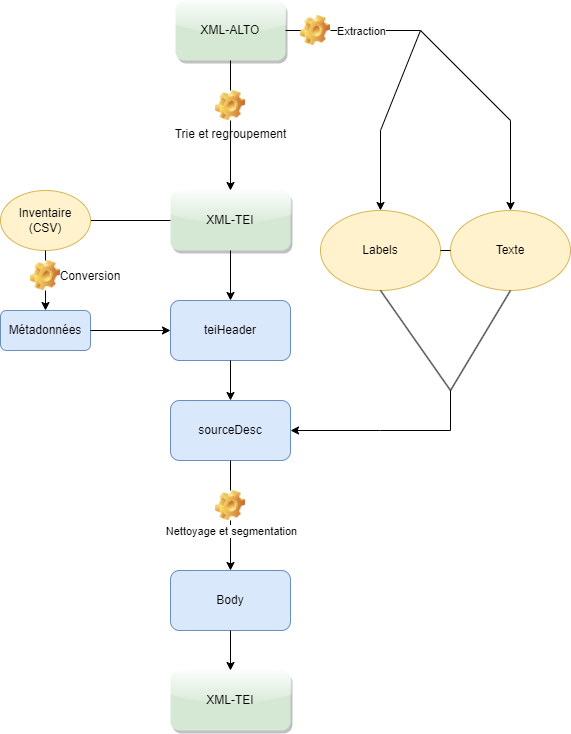
\includegraphics[width=0.7\textwidth]{annexes/schema/altototei.png}
	    \caption{Schéma de conversion des fichiers ALTO vers le format XML-TEI}
	    \label{fig:altototei}
	\end{figure}
	
	Nous avons donc décidé de remanier l'application originale afin d'adopter la structure et la transformation au projet éditorial conçu par le centre \gls{acab}, permettant un gain de temps considérable et fondé sur une une expérience antérieure solide\footnote{application développée pour le projet Araucania est disponible içi. \cite{humeauTeiTransformation2022}}. Comme présenté sur le schéma (voir figure \ref{fig:altototei}), la première étape s'applique à regrouper les fichiers \gls{alto} selon leur identifiant et appliquer la transformation par groupe, en créant la racine \balise{TEI} et de récupérer les labels des régions et des lignes au sein du fichier \gls{alto}. Les différentes métadonnées retranscrites au sein de l'inventaire \gls{csv} sont alors enregistrés au sein du \balise{teiHeader} grâce à la librairie \texttt{Pandas}. Ensuite, le texte contenu dans les \attribut{CONTENT} est extrait des fichiers \gls{alto} et réassocié aux labels précédemment recensés puis structuré selon les pages, les zones puis les lignes au sein du \balise{sourceDesc}. Les données récoltées sont enfin nettoyées et restructurées au sein du \balise{text} en fonction des attributs \attribut{type} et \attribut{subtype} des différentes lignes et des différentes zones afin d'appliquer le schéma éditorial.
	
	\subsection{Documenter et valider un schéma}
	
	Au sein du chapitre 1, nous avons pu constater la variété typologique de notre fonds documentaire et la forte représentativité des sources épistolaires. Pour le moment, le projet c'est avant tout axé sur l'édition de ces documents dont la quantité et la similarité diplomatique justifie une automatisation. Selon l'évolution du traitement du fonds, d'autres schémas pourront être développés.
	
	Afin d'assurer la pérennité de cette édition et le sens sémantique de sa structuration, la conception d'une \gls{ODD} est primordiale puisqu'elle permet de documenter l'ensemble des choix éditoriaux entrepris au cours de cette édition\footnote{La consultation de l'ODD pour la correspondance est consultable au sein du dossier documentation, \cite{humeauTeiTransformation2022}}. Cette documentation devient en quelque sorte le révélateur des enjeux scientifiques, des réflexions éditoriales et de la méthodologie critique du document. Dans notre cas, cette \gls{ODD} à propos de la correspondance a été générée à partir du modèle de transformation \textit{ODD by example} grâce à la création d'un scénario sur le logiciel \texttt{Oxygen} et le processeur Saxon 9. L'\gls{ODD} a par la suite été enrichie manuellement afin de décrire l'encodage utilisé.
	
	\begin{listing}
	        \begin{minted}{xml}
            <constraintSpec scheme="schematron" ident="refVal">
                 <constraint>
                    <s:rule context="tei:placeName[@ref and ancestor::tei:body]">
                        <s:let name="ref" value="@ref"/>
                        <s:assert test="//tei:place[@xml:id = substring-after($ref, '#')] and starts-with($ref, '#')"> The value of @ref has not been declared |<s:value-of select="$ref"/>| </s:assert>
                    </s:rule>
                </constraint>
            </constraintSpec>
            \end{minted}
        	\caption{Application d'une règle \textit{Schematron}}
        	\label{code:schematron}
    \end{listing}
	
	
	
	L'autre enjeu de la construction est la validation et la spécification de notre schéma \gls{tei}. Cette spécification peut se faite grâce aux éléments \balise{schemaSpec}, \balise{moduleRef},\balise{elementSpec} et \balise{classSpec} permettant de modifier la grammaire ou restreindre les règles applicables au schéma \gls{xml}, voir une DTD (Document type definition)\footcite{burnardQuEstceQue2015}. La déclaration de certaines règles \textit{Schematron} a permis de préciser l'usage de certains attributs et de leurs contenus au travers de règles. Comme nous avons pu le voir ci-dessus (voir code \ref{code:schematron}, la règle \textit{Schematron} décrit l'obligation pour tous éléments \balise{placeName} d'avoir son identifiant référencé au sein d'un élément \balise{place} présent au sein du \balise{profileDesc}. La conversion de l'ensemble de ces règles et de cette documentation sous le format \gls{RNG} permet d'automatiser le travail de validation et d'évaluation de la conformité des documents \gls{tei} produits. Cette vérification est exécutée à la fin de l'application du script de conversion avec la fonction de classe \texttt{validate} de la librairie \texttt{lxml}.
	
	\section{Mise en place de l'application autour d'un schéma}
	
	Comme l'amorçait nos premières observations sur l'utilisation d'un script de transformation, la mise en place de cet encodage \gls{tei} nécessite de revenir aux choix employés lors de la production. L'emploi de la libraire \texttt{Lxml} a été indispensable dans l'extraction, la structuration et l'enrichissement des données. 
	
	Ainsi, les axes de nos observations se fondent sur les entités fondamentales de la \gls{tei} : le \balise{teiHeader}, le \balise{sourceDesc} et le \balise{text}.
	
	\subsection{Le teiHeader et ses métadonnées}
	
	Le \balise{teiHeader} correspond à l'élément en-tête d'un fichier XML-TEI. Il regroupe et structure l'ensemble des métadonnées recensées au cours de sa production, permettant d'indexer et de contextualiser le document source. La granularité du schéma des métadonnées doit être ainsi clairement définie en amont en se basant sur la transformation du fichier \gls{alto} lui-même, le ou les documents numériques originelles (facs-similés, ect.) et l'inventaire décrit ultérieurement par la section archivistique du centre \gls{acab}. Le point d'appui pour leurs recensements repose sur l'identifiant extrait du fac-similé numérique afin d'aligner les données avec l'inventaire sous le format \gls{csv}\footcite[voir le fichier ./src/opt/inventory.py ;][]{humeauTeiTransformation2022}.
	
	\begin{figure}[h!]
	    \centering
	    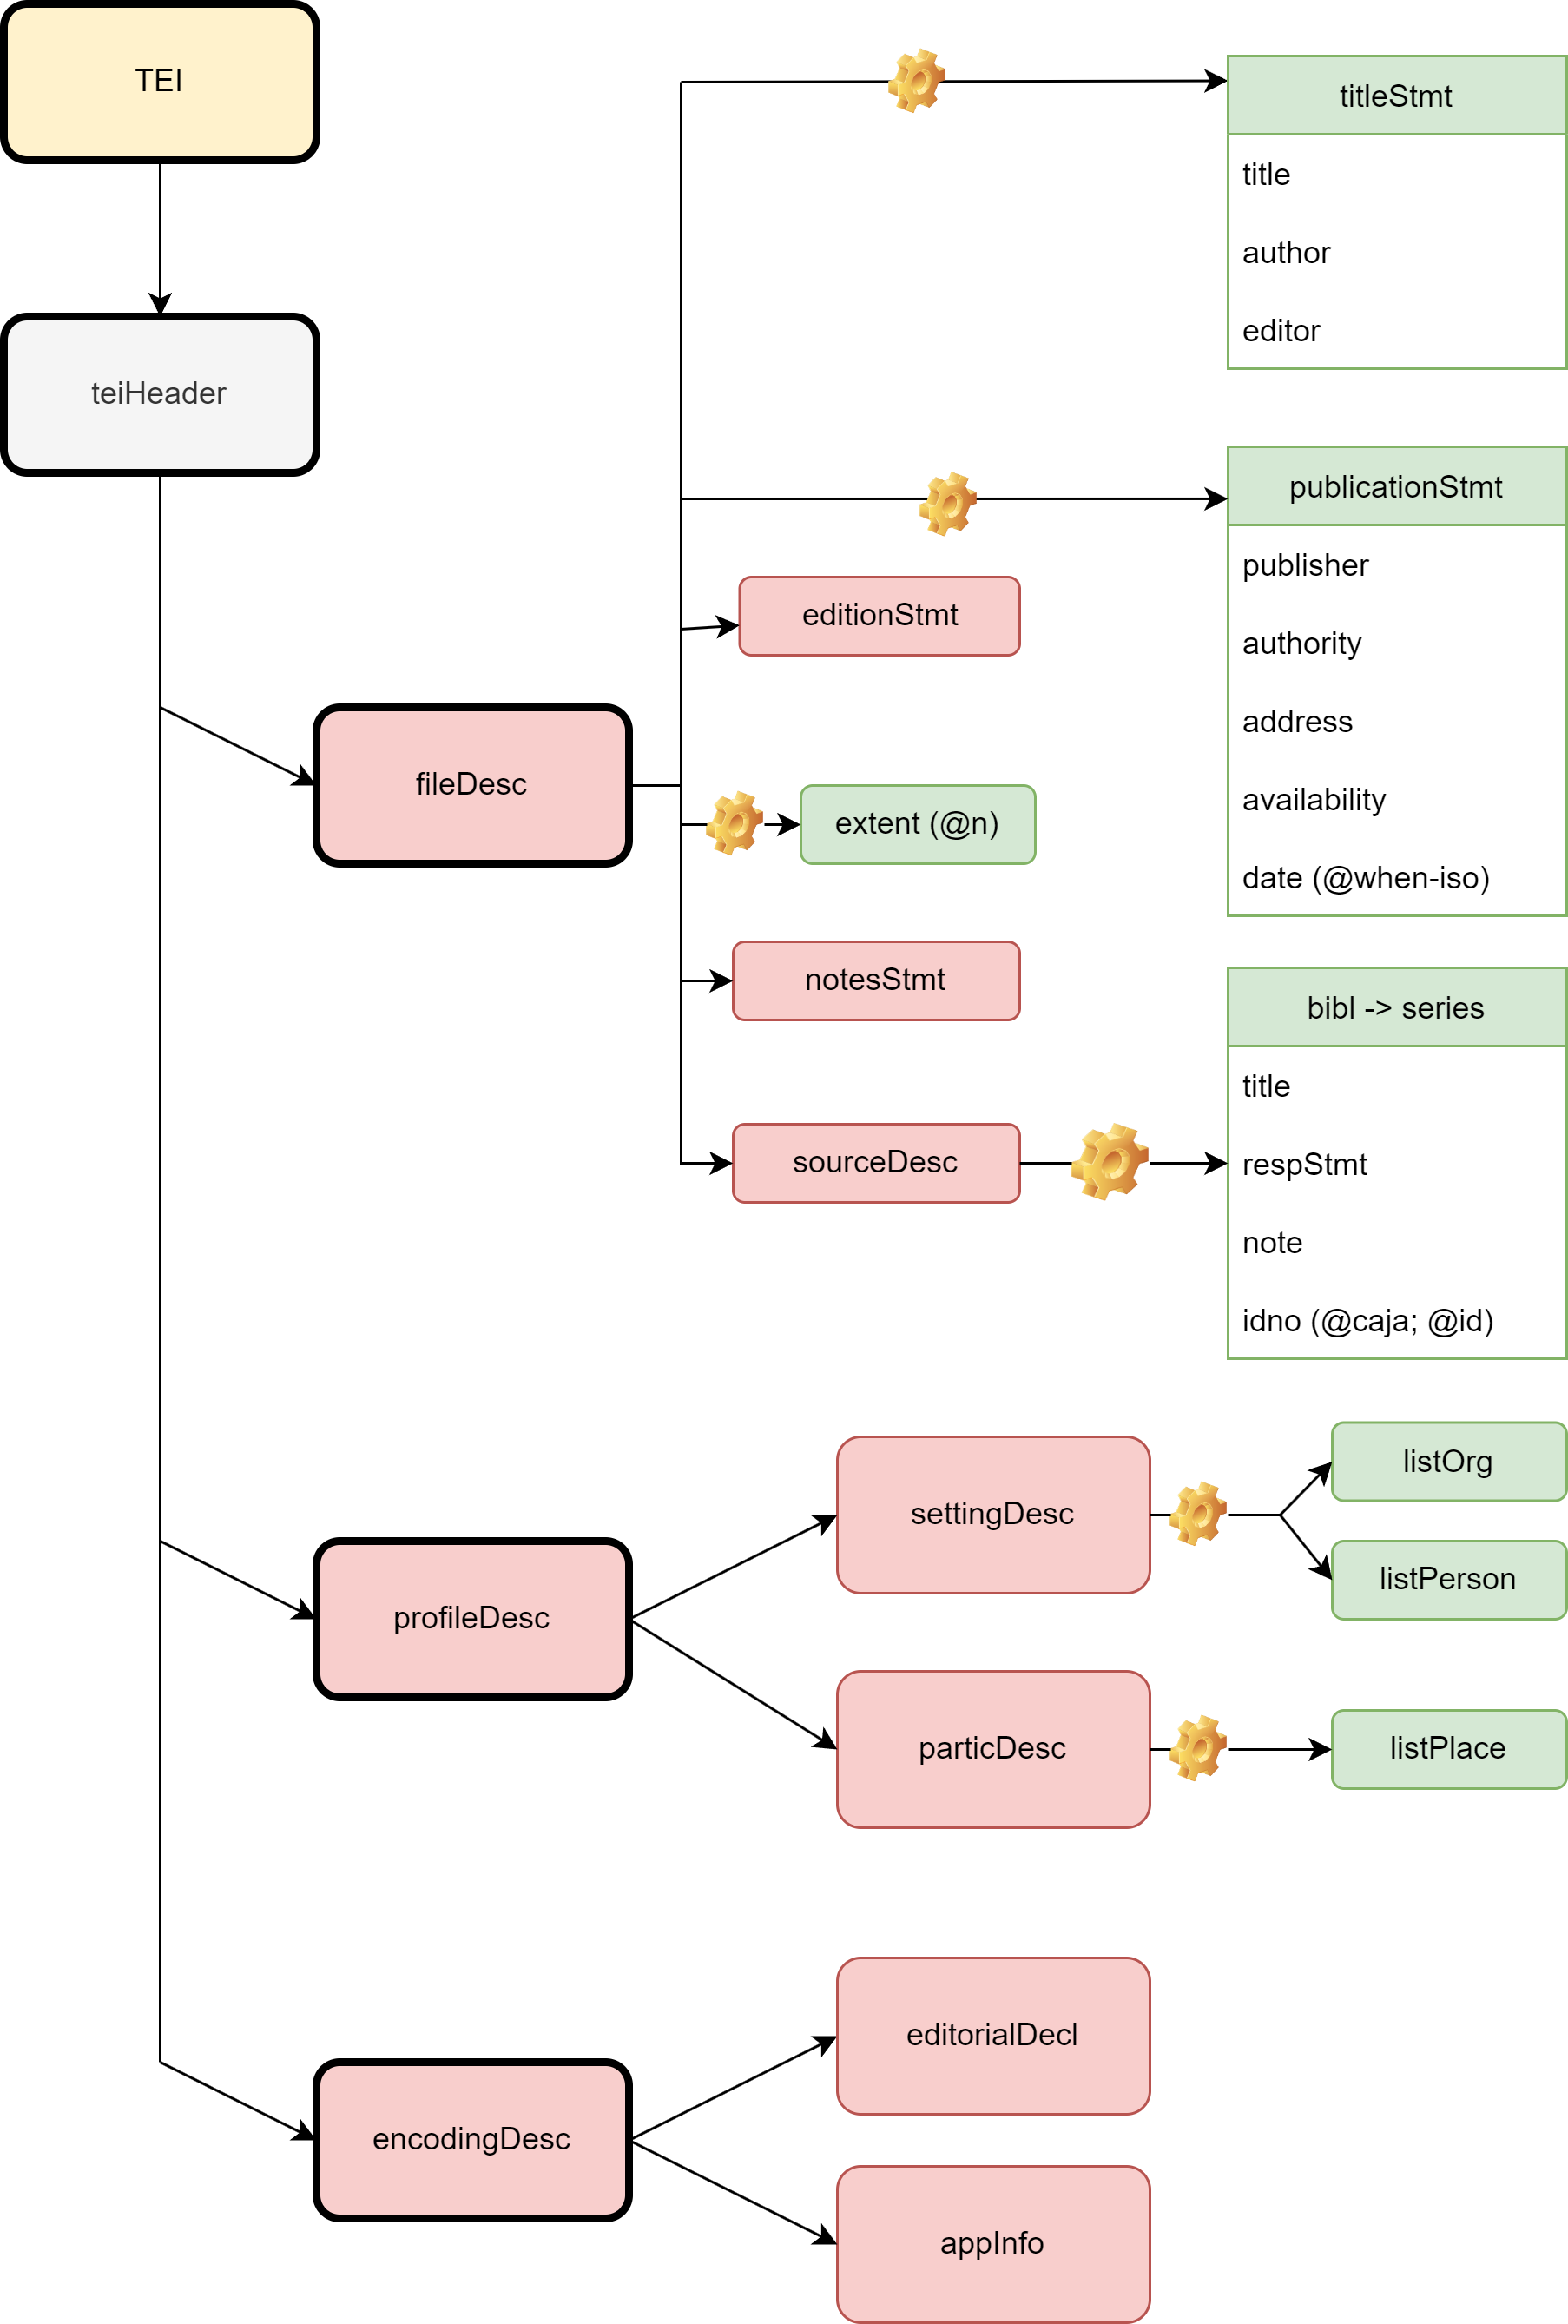
\includegraphics[width=0.7\textwidth]{annexes/schema/teiheader.png}
	    \caption{Structuration du teiHeader}
	    \label{fig:teiheader}
	\end{figure}
	
	Dans un premier temps, les métadonnées décrivent l'ensemble des informations de productions du fichier TEI au sein de l'élément \balise{fileDesc} à partir des métadonnées extraites de l'inventaire\footcite[La structuration de l'arbre du \balise{teiHeader} est disponible en suivant le chemin suivant : ./src/teiheader.py .][]{humeauTeiTransformation2022}. Le \balise{titleStmt} renseigne alors les informations essentielles telles que le titre et l'auteur du document. À l’inverse, les éléments \balise{publicationStmt}, \balise{editionStmt} et \balise{notesStmt} sont pratiquement inamovibles en raison de leur fonction descriptive. Ces balises regroupent les informations de l'autorité éditoriale et de publication. Nous avons choisis de rattacher ces deux éléments à la description du centre \gls{acab} étant, pour le moment, la seule institution véritablement engagée au sein de ce projet d'édition. En revanche, les responsables directs sont identifiables à partir d'un fichier \gls{json} aisément modifiable par les intervenants, puis extrait au cours de la transformation. 
	
	Le décompte des documents rattachés au fichier TEI est décrit au sein de l'élément \balise{extent} affichant la quantité de fac-similés dénombrés sous cet identifiant, avant d'être identifié au sein du \balise{sourceDesc} décrivant le fonds documentaire de l'Araucania. Les métadonnées d'ordre technique sont davantage disposées au sein du \balise{encodingDesc} permettant de décrire succinctement les pratiques autour de cet encodage. L'élément \balise{appinfo} permet de détailler les différentes applications utilisées sur l'ensemble de la chaîne de traitement. Cette description permet de renforcer l'usabilité et la compréhension des données édités en retraçant l'ensemble des processus subit au sein du fichier électronique.

	\subsection{\balise{sourceDoc} : une trace originale}
	
	Dans sa définition officielle, le \balise{sourceDoc} est un élément qui contient une transcription ou autre représentation d'un document source unique faisant potentiellement partie d'un dossier génétique ou d'une collection de sources. Plus concrètement, cet élément devient le lieu de description du fichier \gls{alto} d'origine en reprenant les éléments de mise en page et du texte océrisé. La structuration est directement reprise depuis le modèle établi par l'application \texttt{Alto2tei}\footcite{christensenAlto2tei2022}.
	
	\begin{listing}
	\begin{minted}{xml}
	<surfaceGrp>
      <surface xml:id="299_a" n="16" ulx="0" uly="0" lrx="2327" lry="2970">
        <graphic url="./input/299_a.jpg"/>
        <zone xml:id="299_a_z1" type="CustomZone" subtype="Dateline" n="1" points="1515,217 [...] 1128,178 1294,178 1425,247" source="./input/299_a.jpg" corresp="eSc_textblock_18faefaf">
          <zone xml:id="299_a_z1_l1" type="DefaultLine" subtype="none" n="1" points="1037,388 1133,413 [...] 1034,289 1037,348" source="./input/299_a.jpg" corresp="eSc_line_d13c289a">
            <path xml:id="299_a_z1_l1_p" points="1037,348 [...] 1953,334"/>
            <line xml:id="299_a_z1_l1_t">⁋Valparaiso, Julio 101860</line>
          </zone>
    [...]
    </surface>
    </surfaceGrp>
	\end{minted}
	\caption{Exemple de structuration du sourceDoc}
	\label{code:sourcedoc}
	\end{listing}
	
	En observant plus attentivement, la structuration est une réadaptation du modèle ALTO vers l'encodage TEI en reprenant les données essentielles. L'ensemble des fac-similés numérisés est ainsi décrit au sein de l'élément \balise{surface} en rassemblant l'ensemble des zones et des lignes rattachées. Elles sont décrites au sein de la balise \balise{zone} dont les types et les sous-types issus d'une segmentation préalable indiquent la typologie\footnote{CustomZone:Dateline est décousu en deux attributs : type='CustomZone' et subtype="Dateline")}. L'ensemble des coordonnées ALTO ont été conservées au sein des \attribut{points}, laissant ainsi la possibilité d'exploiter ses coordonnées directement au sein de l'image numérisée. Enfin le contenu textuel est identifiable parmi l'élément \balise{line} et le masque \gls{htr} associé, présent dans l'élément précédent \balise{path}.
	
	La bonne extraction et l'attention particulière à la propreté et la validité des données sont fondamentales puisqu'elles constituent la base de la future structuration du \balise{text}. Du reste, cette conservation exhaustive des données initiales accorde une grande facilité à entretenir l'interopérabilité et la pérennité des éditions numériques, et ainsi leurs réexploitations.
	
	\subsection{Structurer et éditer un texte}
	
	Comme nous l'avons vu au cours du chapitre 1, la définition d'une ontologie et la mise en corrélation avec le vocabulaire contrôle \textit{SegmOnto} au cours du processus de transcription automatique a permis de conserver la valeur sémantique et sémiotique de l'image originale. Cette structuration en amont a ainsi constitué l'arc de voûte de la transformation et l'adaptation de l'\gls{alto} à l'encodage \gls{tei}. À partir de là, l'extraction des différents labels présents au sein du fichier \gls{alto} nous permet d'organiser la structuration du texte en fonction des différentes zones et des différentes lignes présentes.
	
	Au sein de l'élément \balise{text}, il nous faut établir deux subdivisions entre le \balise{body} qui représente le contenu initial du document et le groupe \balise{noteGrp} permettant d'y recenser la plupart des écrits ultérieurs. Seules les lignes contenues au sein d'une zone \textit{NumberingZone} sont référencées au sein de la balise \balise{fw}, à l'intérieur du \balise{body}, indiquant des éléments de mises en pages\footnote{Hormis le sous-groupe \textit{id} qui rejoint les notes postscript}. La seconde étape consiste à repérer le commencement d'une nouvelle page en se référant au numéro de ligne. Si elle est la première, elle indique la présence d'une nouvelle page soulignée par l'incrémentation de l'élément \balise{pb} et son identifiant au sein \attribut{corresp}.
	
	\begin{figure}
	    \centering
	    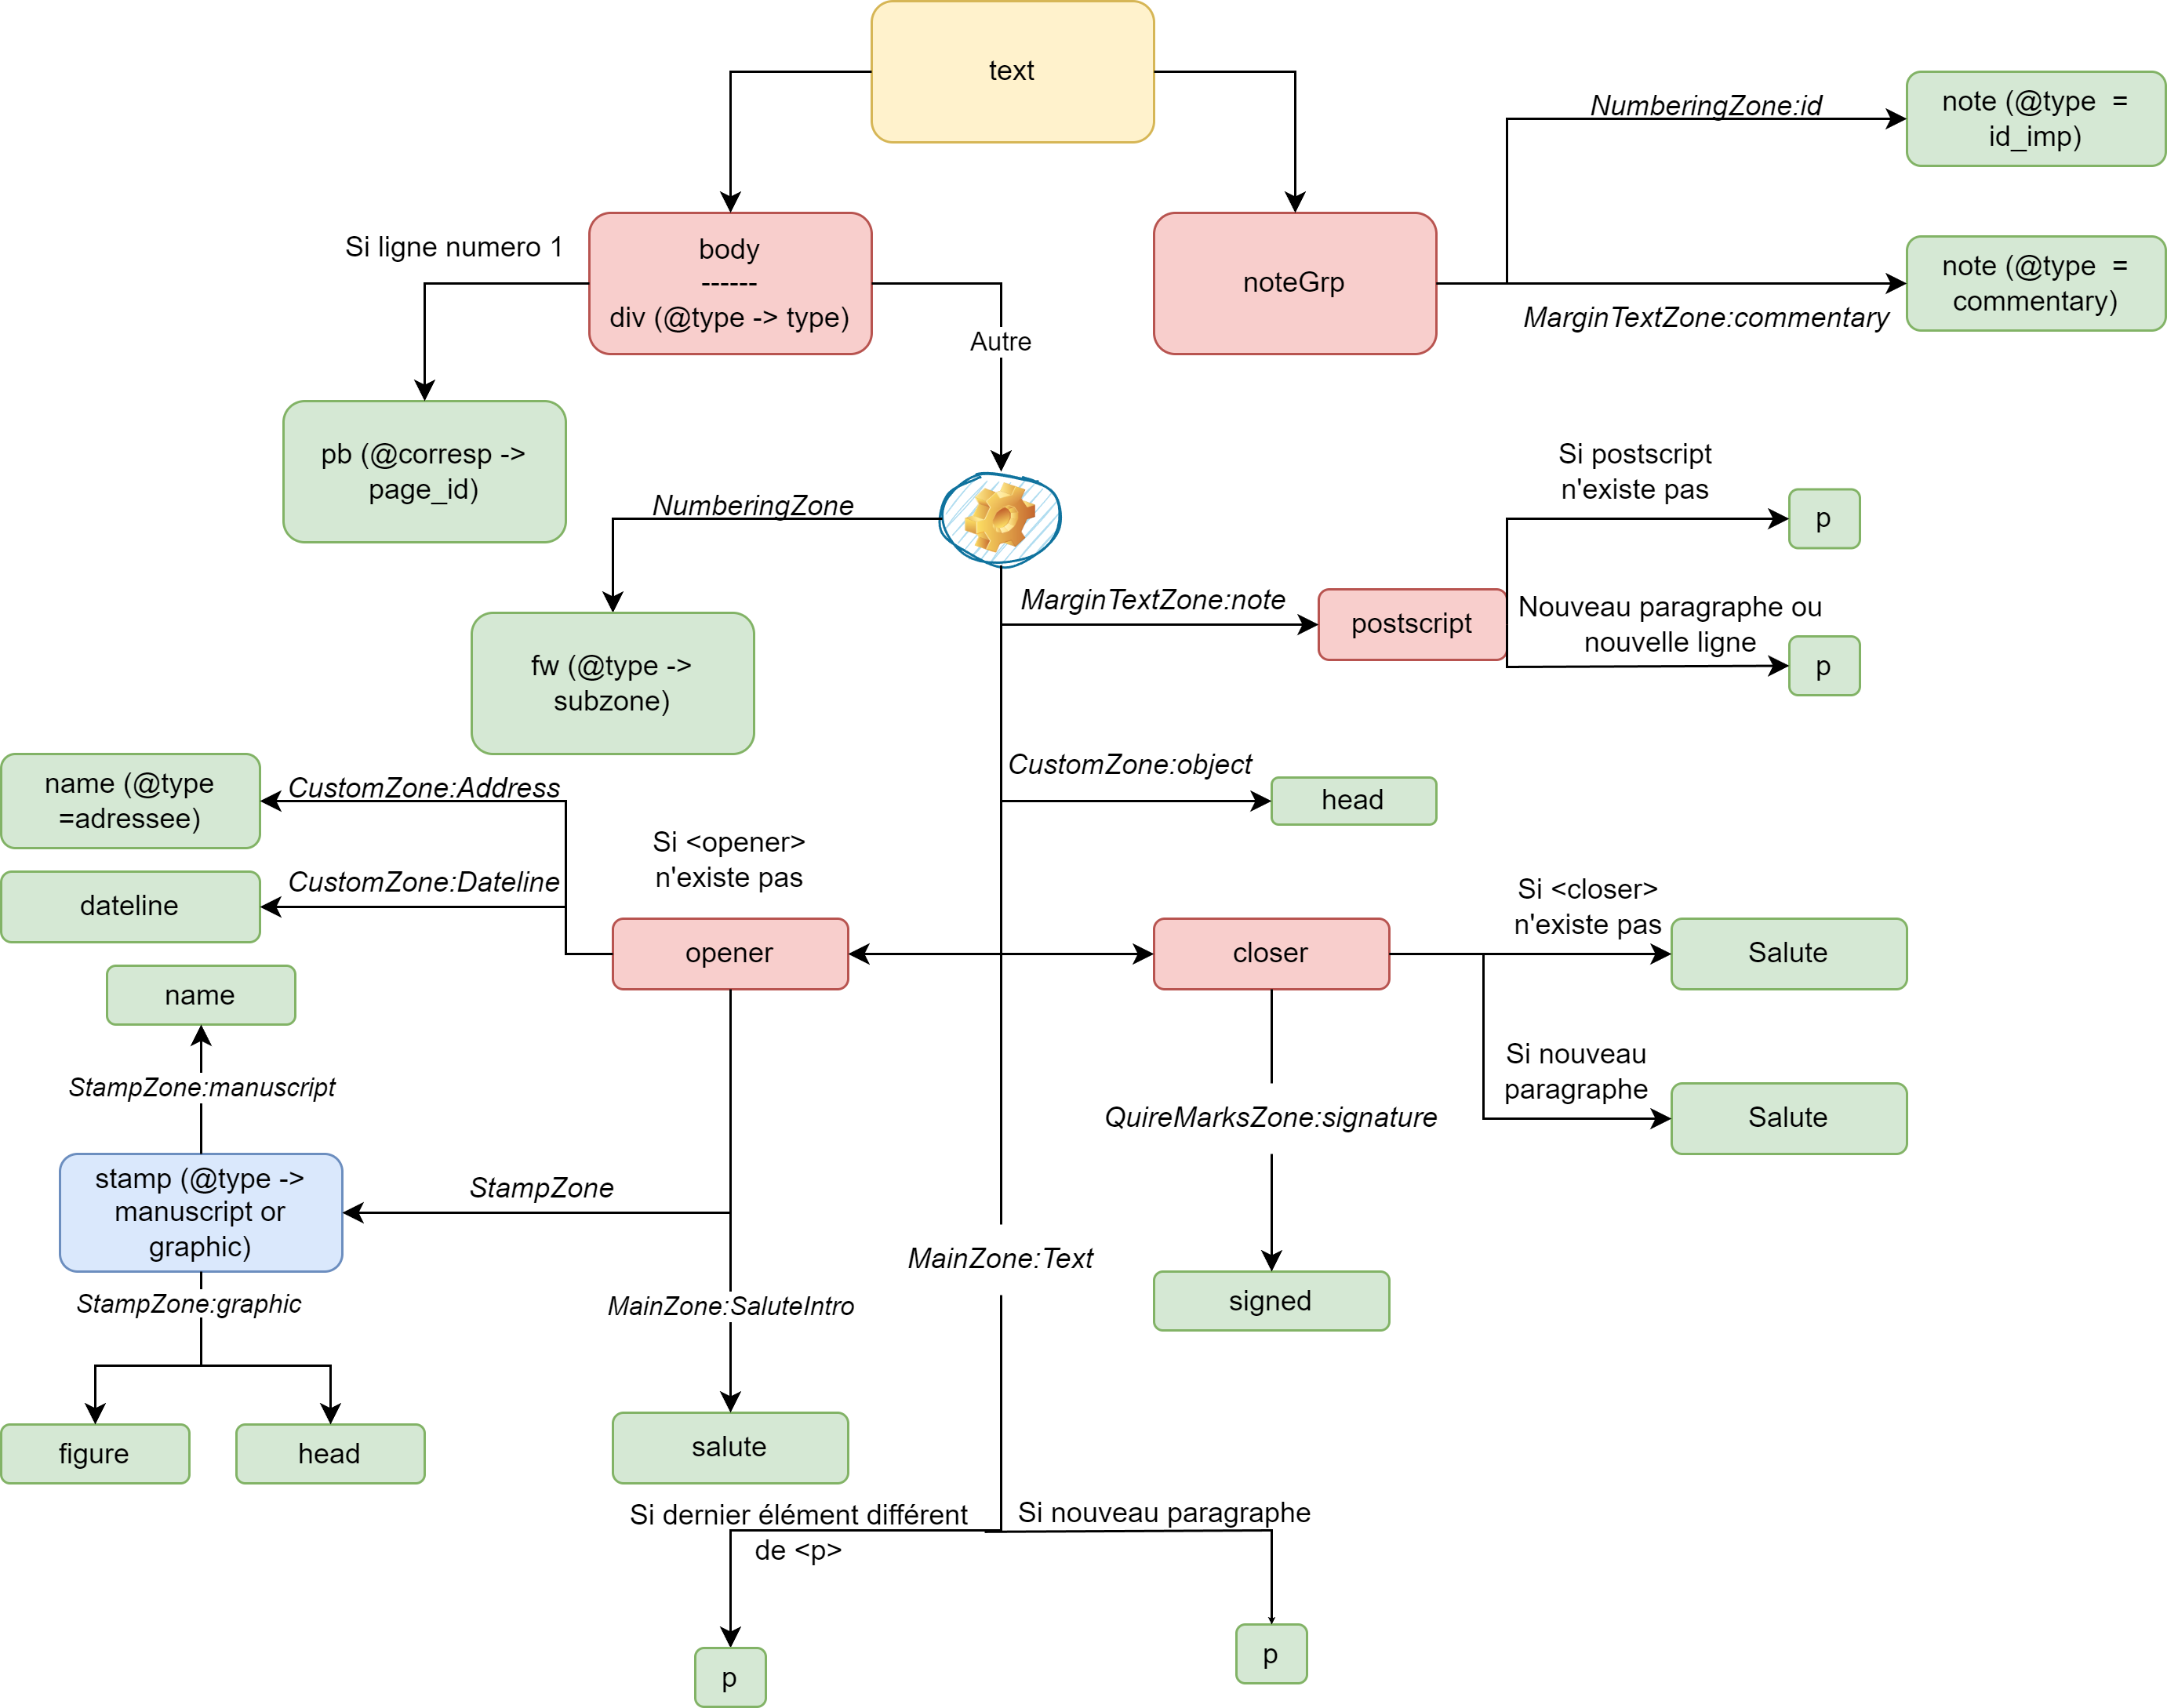
\includegraphics[width=1\textwidth]{annexes/schema/decision_body.png}
	    \caption{Arbre décisionnel de structuration de \balise{text}}
	    \label{fig:arbre_texte}
	\end{figure}
	
	Le schéma et la granularité du \balise{body} sont ainsi organisés en fonction de l'ontologie \gls{htr} développée précédemment. Ce schéma reprend les recommandations du modèle établi pour l'édition de la correspondance de l'édition \gls{dahn}\footcite{chiffoleauDAHNProjectDigital2022}. Ce \balise{body} est en réalité subdivisé en 3 sections majeures et une section optionnelle:
	\begin{itemize}
	    \item \balise{opener} regroupe l'ensemble du discours introductif et les éléments de contextualisation présentés par l'auteur. Il comprend les ontologies \gls{segmonto} suivantes : les éléments \textit{StampZone}, les sous-groupes \textit{CustomZone} comprenant l'adresse, la date (spatiale et temporelle) et la salutation introductive présente au sein du label \textit{MainZone:SaluteIntro}.
	    \item A l'inverse, le \balise{closer} représente l'élément général de conclusion du document. Il rassemble le salut final, parfois sectionné, et la suscription de l'auteur vers son homologue.
	    \item Le corps principal du texte est quant à lui directement injecté au sein du \balise{body} à travers l'élément \balise{p}. Lors de l'énumération des différentes lignes du sourceDoc présentes au sein du \textit{MainZone:text}, la rencontre du signe '\P' signale un nouveau paragraphe qui est alors décompté.
	    \item La mise en place d'un élément \balise{postscript} est parfois nécessaire, en raison de la présence d'une zone possédant le label \textit{MarginTextZone}. Ces notes marginales au texte principal peuvent être divisées en différents paragraphes selon leurs mises en pages. \newline
	\end{itemize}
	
	Cette structuration n'est pas totalement représentative de la mise en page du fac-similé original en raison de la propriété \textit{tail}, mise en place avec la librairie \texttt{Lxml}.  De cette façon, l'\gls{API} \textit{ElementTree} ne nécessite pas de nœuds de texte spéciaux en plus de la classe \textit{Element}, qui ont  parfois tendance à se mettre en travers du chemin. L'inclusion d'une balise autofermante \balise{lb} permet de signaler la présence d'une nouvelle ligne sans déformer la structuration initiale. Cette technique permet de plus facilement ingérer ou modifier le fichier \textit{a posteriori}\footnote{Voir le site web de la librarie Lxml : \textit{Lxml}, url: \url{https://lxml.de/tutorial.html}, consulté le 21/08/2022.}.
	
	Une telle structuration souhaite ainsi répondre aux besoins d'intelligibilité et d'interropérabilité des données éditées comme le rappel l'ingénieur Syd Bauman\footnote{Syd Bauman, \enquote{Interchange vs. Interoperability} In \textit{Balisage: The Markup Conference 2011 Proceedings}, Montréal, 2011 \textit{via} \cite{munozTextsDocumentsNew2014}}. Elle doit faire ressortir aisément les identités du texte à la fois pour l'œil  humain et la machine. L'automatisation de ces éditions renforce ainsi cette accessibilité en facilitant le futur traitement et la future exploitation du fichier TEI édité.
	%%%%%%% CORRECTION DONE %%%%%%%%%%
	
	%%%%%%%%%%%% CHAPTER 4 %%%%%%%%%%%%%%%%%
	\chapter{Indexer et enrichir une édition numérique}
	
	Alors que les humanités numériques, évoquées au travers de la philologie, incarnent un progrès méthodologique considérable pour le travail en amont, Jean-Baptiste Camps rappelle que cette mise en place d' une édition numérique reste un effort fastidieux, chronophage et coûteux pour les institutions\footcite{campsOuVaPhilologie2018}. Si la sérialisation des données ne peut-être une fin en soi, l'enrichissement des textes, primordial à la recherche, peut tout de même être considérablement allégé grâce à l'ingénierie.
	
	Aujourd'hui, les outils associés au traitement automatique des langues sont devenus suffisamment matures et fiables pour fournir une analyse à la fois quantitative et qualitative. Ces avancées ont permis de créer un véritable engoument du \gls{tal} au sein des humanités numériques et de l'édition numérique\footcite{mcgillivrayDigitalHumanitiesNatural2020}. De nombreux écosystèmes ont été développés dans le but de permettre un enrichissement quantitatif de bases de données XML-TEI à partir de la fouille de texte et l'extraction de l'information\footcite{bissonNoticesAutoriteXMLTEI2020}. Ces différents processus permettent régulièrement la correction des données produites par les modèles \gls{htr}\footnote{Nous l'avons partiellement vu avec la mise en place d'une application correctrice au travers de l'algorithme de Levenshtein}, l'indexation des entités ou encore de faciliter la recherche au sein du texte\footcite{terrielRepresenterEvaluerDonnees2020}.
	
	Durant ce projet d'édition des archives de l'Occupation de l'Araucania, l'implantation d'un système d'enrichissement fondé sur les concepts du traitement automatique du langage et la reconnaissance d’entités nommées a été un des axes majeurs du processus éditorial. La mise en place d'un tel procédé nécessite de revenir sur les enjeux épistémologiques et techniques d'un processus lourd et complexe. Dans ce cadre, nous allons observer au cours de ce chapitre les différentes réflexions et observations qui ont accompagné et nourrie cette insertion technique d'un pré-enrichissement automatique.
	
	
	\section{L'ébullition du traitement du langage naturel}
	
	Pour comprendre les progrès qui ont entouré l'incorporation du \gls{tal} dans le domaine des humanités numériques, il est nécessaire d'en décliner les principes généraux et les innovations récentes permises par la généralisation du \textit{deep learning} et des nouvelles architectures affiliés.
	
	En ce sens cette partie se veut comme un aparté pédagogique et introductif autant sur le plan théorique que technique.
	
	\subsection{Principes généraux du TAL}
	
	Le traitement automatique des langues est en réalité une discipline regroupant un ensemble de pratiques autour de l'analyse et l'interprétation des langues naturelles à travers l'outil informatique. Ce domaine pluridisciplinaire est ainsi à la croisée de la linguistique, de l’informatique, des mathématiques et de l’intelligence artificielle. Aujourd'hui, le \gls{tal} regroupe un ensemble de technologies de la vie courante et scientifique tel que les traducteurs automatiques, l'analyse marketing et des sentiments, le \textit{data mining} (fouille de texte, en français), la correction orthographique, la reconnaissance vocale, etc... Quatre catégories peuvent être définies : le traitement syntaxique et sémantique, l'extraction d'information et le traitement du signal\footnote{Cette catégorisation reprend la déclinaison faite au sein de la page Wikipedia dédiée au \gls{tal}. \textit{Wikipidia | Traitement automatique des langues}, url: \url{https://fr.wikipedia.org/wiki/Traitement_automatique_des_langues}, consulté le 20/08/2022.}.
	
	Le \gls{tal} provient d'un très long processus de recherche remontant aux débuts des années 1960 avec un véritable engouement probabiliste à partir des années 1983 et 1984\footcite[Cette éclosion d'intérêt au sein des milieux scientifiques est permis avec la publication des premiers arbres de décisions et de d'un système d'étiquetage probabiliste.][]{tanguyEvolutionsLinguistiqueOutillee2014}. Dans un article paru en 2014, Ludovic Tanguy y distingue deux méthodes : la première dite \enquote{traditionnelle} ou linguistique consistant à formaliser les règles à appliquer et les ressources linguistiques. La seconde réside dans la mise en place de modèles mathématiques et statistiques applicables à l'intelligence artificielle\footcite{tanguyEvolutionsLinguistiqueOutillee2014}.
	
	À l’heure actuelle, ce domaine de l'apprentissage machine s'appuie sur un ensemble de pratiques syntaxo-sémantiques bien précises, bâtit autour des modèles linguistiques, dont les principales fonctionnalités sont les suivantes :
	\begin{itemize}
	    \item La tokenisation qui consiste en la segmentation d'une phrase en mot ou d'un mot en caractères.
	    \item Le \textit{stemming} et la lemmatisation. La première technique désigne le découpage de la fin du mot pour en conserver la racine. La lemmatisation consiste quant à elle à supprimer les terminaisons \enquote{en isolant la forme canonique du mot\footcite{labbeNormalisationLemmatisationQuestion}}.
	    \item L’étiquetage morpho-syntaxique (POS) est un processus reliant le mot à sa fonction grammaticale.
	    \item La suppression des mots vides (\textit{stop words} en anglais), c’est-à-dire les mots courants et vides de sens propres.
	    \item Le Plongement de mots ou lexical (\textit{word embbeding} en anglais) est une méthode de représentation d'un mot sous forme de vecteur. Elle donne une valeur numérique au sens et au contexte du mot en établissant un vecteur contextuel.
	\end{itemize}
	
	\subsection{Les réseaux neuronaux et le TAL : la révolution des modèles encodeurs-decodeurs}
	
	Aujourd'hui, le \gls{tal} s'est totalement inséré dans nos vies quotidiennes avec la renaissance du \textit{machine learning}, après la crise qu'il a connu au cours des années 2000. Plus particulièrement, cette démocratisation a été permise par l'amélioration notable des performances avec l'utilisation du \textit{deep learning}. Ces dernières avancées ont su puiser dans l'approche du \textit{Word Embbeding} afin de constituer des algorithmes statiques au texte à l'image du système \textit{Word2Vec}, notamment le modèle Skip-Gram\footcite[D'autres valorisent des approches moins lourdes de plongement de mots tel que le \textit{Singular Value Decomposition}][]{moodyStopUsingWord2vec2017}. 
	
	En 1957, le linguiste John Rupert Firth émet l'hypothèse suivante : \enquote{You shall know a word by the compagny it keeps !\footnote{\enquote{Vous reconnaîtrez un mot à la compagnie qu'il garde !} in \cite{widdowsonFirth1957Papers2007}}}. Cette hypothèse distributionnelle qui reconnaît un mot à partir de son contexte va être le socle du système \textit{Word2Vec}. Alors, l'algorithme de transformation vers des valeurs algébriques tend à étendre la définition originale de la distribution en y incluant une valeur sémantique et contextuelle au travers d'espaces multidimensionnels. La distance vectorielle indique ainsi la proximité sémantique entre deux mots. Ces transformations des mots sous des modèles algébriques (matriciels et vectoriels) permettent ainsi de définir les poids des réseaux neuronaux appliqués.
	
	\begin{figure}[h!]
	    \centering
	    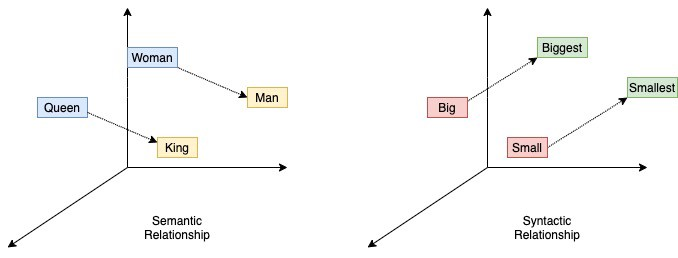
\includegraphics[width = 0.7\textwidth]{annexes/img/word_embedding.jpeg}
	    \caption{Représentation vectorielle des relations sémantiques et syntaxiques - \copyright towardsdatascience, 2021}
	    \label{fig:word_embedding}
	\end{figure}
	
	Afin de traiter les données en séries, deux architectures neuronales sont principalement utilisés; les premiers furent les réseaux neuronaux acycliques (RNN ; LSTM et GRU), aujourd'hui dépassés en raison des problèmes de \enquote{rétropropagation}\footcite[p.~161]{clericeDetectionIsotopiesPar2022}. C'est-à-dire que l'algorithme concentre davantage son attention sur la fin d'un élément. Ce phénomène est réglé par les réseaux \gls{CNN} en prenant l'élément dans sa globalité\footcite[p.~164]{clericeDetectionIsotopiesPar2022}. Ce réseau s'exerce en deux étapes : la partie convolutive qui se tâche de l'extraction des caractéristiques propres à travers différents algorithmes de transformation (\textit{pooling}, échantillonage, etc...), puis la classification des données.
	
	Depuis la fin des années 2010, le \gls{tal} s'est dirigé vers les architectures encodeurs-décodeurs. Cette innovation se fonde sur les réseaux acyliques et l'application du mécanisme de l'attention, du système \textit{Masked LM}, l'application d'un masque aléatoire permettant une approche simultanée du traitement, et l'approche du \textit{Dynamic Embedding}\footcite{vaswaniAttentionAllYou2017}. En 2018, Google présente le modèle BERT (\textit{Bidirectional Encoder Representations from Transformers}) qui étalonne en de multiples étapes cycliques le traitement textuel \textit{via} une architecture encodeur-décodeur\footcite{devlinBERTPretrainingDeep2019a}. Ces modèles de langage appellent plus couramment appelés modèles \textit{Transformers}. Ces modèles de langages sont des outils de pré-entraînement de modèles plus perfectionnés, à travers la méthode du \textit{fine-tuning}.
	
	De nombreux modèles de langage ont fait leurs apparitions à la suite de cette révolution au sein du \gls{tal} et la démocratisation des modèles \textit{Transformers}\footnote{Il est à noter que cette architecture démontre aussi des capacités prometteuses pour le cas de la reconnaissance d'écriture. \cite{kassAttentionHTRHandwrittenText2022}}. En 2020, l'Universidad de Chile développe et publie le modèle BETO qui reprend les principes de cette architecture pour l'adapter à la langue espagnole, en utilisant la méthode du \textit{fine-tuning} avec le modèle BERT \footcite{caneteSpanishPreTrainedBERT2020}. Le \textit{dataset} a été constitué à partir des données de Wikipedia et du projet OPUS. Comme l'indique le tableau \ref{tab:beto_benchmarlk}, les résultats du modèle sont très satisfaisants, plus particulièrement pour le modèle prenant en compte la case dans son analyse. Ce modèle constituera notre point d'appui pour le développement du projet d'enrichissement de nos éditions numériques.
	
    \begin{table}[]
    \begin{tabular}{|c|r|r|r|}
    \hline
    \textbf{TASK} & \multicolumn{1}{c|}{\href{https://huggingface.co/dccuchile/bert-base-spanish-wwm-cased}{\textbf{BETO-cased}}} & \multicolumn{1}{c|}{\href{https://huggingface.co/dccuchile/bert-base-spanish-wwm-uncased}{\textbf{BETO-uncased}}} & \multicolumn{1}{c|}{\href{https://huggingface.co/bert-base-uncased}{\textbf{Best Multilingual BERT}}} \\ \hline
    \href{https://lindat.mff.cuni.cz/repository/xmlui/handle/11234/1-1827}{POS}           & 98.97                                    & 98.44                                      & 97.10                                                \\ \cline{1-1}
    \href{https://www.kaggle.com/datasets/nltkdata/conll-corpora}{NER-C}         & 55.43                                    & 82.67                                      & 87.38                                                \\ \cline{1-1}
    \href{https://github.com/facebookresearch/MLDoc}{MLDoc}         & 95.60                                    & 96.12                                      & 95.70                                                \\ \cline{1-1}
    \href{https://github.com/google-research-datasets/paws/tree/master/pawsx}{PAWS-X}        & 89.05                                    & 89.55                                      & 90.70                                                \\ \cline{1-1}
    \href{https://github.com/facebookresearch/XNLI}{XNLI}          & 82.01                                    & 80.15                                      & 78.50                                                \\ \cline{1-1} \hline
    \end{tabular}
    \caption{Évaluation des performances du modèle BETO (selon standard GLUE)}
    \label{tab:beto_benchmarlk}
    \end{table}
	
    \subsection{Le TAL, la reconnaissance des entités nommées et les humanités}
    
    L'extraction d'information est une catégorie générale de la linguistique computationnelle dont le principe repose sur l'analyse, une sélection et une classification pertinentes d'une donnée textuelle\footcite{poibeauExtractionInformationNouvelle1999}. Elle regroupe de nombreuses tâches permettant de déstructurer et reconstruire l'information telle que l'identification des relations et des évènements, l'extraction de propriétés, la résolution des coréférences ou dans ce qui nous concerne, la reconnaissance des entités nommées.
    
    Le concept linguistique des entités nommées définit le principe d'une classification des mots selon son fonctionnement référentiel. Dans sa thèse sur les processus d'extractions des entités nommées, Maud Ehrmann les décrit comme \enquote{Étant donné un modèle applicatif et un corpus, on appelle entité nommée toute expression linguistique qui réfère à une entité unique du modèle de manière autonome dans le corpus.\footcite[p.~167-168]{ehrmannEntiteesNommeesLinguistique2008}}. Cette définition décrit des propriétés malléables dépendantes d'une ontologie définie préalablement, dont la référence sémantique est alors primordiale et la référence syntaxique secondaire (exemple : les noms propres). Autrement dit, la nature d'une entité nommée ne réside pas dans son essence, mais bien dans son existence applicative\footcite[p.~167-168]{ehrmannEntiteesNommeesLinguistique2008}.
    
    \begin{figure}
        \centering
        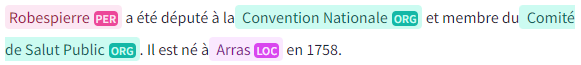
\includegraphics[width=0.6\textwidth]{annexes/img/entites.png}
        \caption{Exemple de reconnaissance d'entités nommées à partir du modèle camemBERT}
        \label{fig:entités}
    \end{figure}
    
    Comme le présente la figure \ref{fig:entités}, la reconnaissance d'entités nommées est une technique consistant à repérer ces chaînes de caractères au sein d'un texte et d'en déterminer son référentiel. Ici, l'ontologie employée se décline en quatre grandes natures : \texttt{LOC} pour les lieux géographiques, \texttt{ORG} pour les organisations, \texttt{PERS} pour les personnes et \texttt{MISC} pour les entités diverses et regroupées au sein de cette catégorie générale (non référencée dans notre cas). Cette approche de classification est parmi les plus communes puisqu'elle reprend les règles définit par CoNLL 2003, une conférence annuelle organisée par la SIGNLL (\textit{ACL's Special Interest Group on Natural Language Learning})\footcite{lemmensCoNLL2022CoNLL2022}. Toutefois, cette normalisation ne peut faire l'objet d'un véritable consensus puisque l'étiquetage reste dépendant des sujets traités en prenant en compte les limites, la porté et la granuralité d'une entité\footcite{hengchenExtractionEntitesNommees2015}.
    
    \subsubsection{Les techniques de reconnaissances des entités nommées}
    
    Le processus de reconnaissance des entités nommées peut s'exercer à travers deux approches techniques, non nécessairement dichotomiques. La première est l'étiquetage des entités par l'intervention humaine en définissant des règles appliquées à partir d'une ontologie préalable. 
    
    Cette méthode majoritairement répandue dans les années 1990 est décrite comme la mise en forme de \enquote{patrons d'extraction} en exploitant les indices morpho-syntaxique et un ensemble de ressources externes\footcite[p.~32]{ehrmannEntiteesNommeesLinguistique2008}. Pour reprendre l'exemple de Maud Ehrmann, si Maximilien est un nom connu au sein des ressources utilisées et que le nom suivant Robespierre est inconnu, mais qu'il possède une majuscule et suit la première entité; alors l'approche statistique peut facilement déduire que Robespierre appartient à l'entité \texttt{PERS}\footcite[p.~33]{ehrmannEntiteesNommeesLinguistique2008}. Toutefois, la mise en place de motifs probabilistes reste parfois insuffisant en raison d'un paramétrage intrinsèquement trop large comme le signale Damien Nouvel\footcite[p.~146]{nouvelReconnaissanceEntitesNommees2012}.
    
    Cette approche a été confortée avec l'utilisation de l'intelligence artificielle qui connaît un nouveau souffle après les années 2000. Elle nécessite l'emploi d'une base de données afin de pouvoir y entraîner différents modèles. Parmi les approches courantes, on peut y recenser :
    \begin{itemize}
        \item L'apprentissage non-supervisé en utilisant des techniques de \textit{clustering}, c'est-à-dire de regroupement de données selon une interprétation machine\footcite{liSurveyDeepLearning2020}.
        \item L'apprentissage supervisé, utilisant donc des données préalablement étiquetées dont les principaux algorithmes utilisés sont les arbres de décisions, le \textit{Machine Support Vector} (SVM) ou le système Markov caché\footcite{liSurveyDeepLearning2020}. Ces modèles sont assez similaires aux modèles classiques de \gls{htr}.
        \item Les algorithmes d'apprentissages profonds se sont imposés comme l'architecture dominante depuis ces dernières années dans les taches de reconnaissances d'entités nommées\footcite{liSurveyDeepLearning2020}. L'ébullition des architectures \textit{Transformers} a amplifié ce phénomène en raison de ces résultats (voir tableau \ref{tab:beto_benchmarlk}). De plus, l'apprentissage profond permet de traiter facilement des données complexes et l'obtention d'un modèle multi-tâche, facilement intégrable au sein d'une chaîne de traitement.
    \end{itemize}
    
    \subsubsection{La REN et les humanités}
    
    L'intégration des technologies \gls{ren} a susciter de nombreux émois au sein des secteurs patrimoniaux et des humanités. La place de plus en plus grande qu'occupent les humanités numériques au sein de la recherche a multiplié l'intérêt pour cette tâche. La préparation de données statiques ou le renouveau historiographique permis par la méthode de \textit{Distant reading}\footnote{Méthode d'analyse historique imaginé par Franco Moretti. Elle consiste en l'application des méthodes calculs et d'observations de motifs à l'échelle de grandes bases de données. \cite{purenLectureDistanteIntroduction2020a}} ont généralisée la fouille de texte, dont l'extraction des entités nommées permet une annotation efficace des documents.
    
    Dans le même temps, le catalogage et l’indexation manuel sont mis à rude épreuve depuis plusieurs années en raison des restrictions budgétaires au sein des secteurs culturels et la multiplication des documents archivés\footcite{hengchenExtractionEntitesNommees2015}. Face à ce constat, les institutions patrimoniales s'essayent à réoganiser le processus d'indexation avec une utilisation systémique des technologies \gls{ren}. Le projet NER4Archives développés par les Archives Nationales en partenariat avec l'\gls{inria} démontre cette volonté d'automatiser la classification au sein des instruments de recherche archivistique\footcite{clavaudNER4ArchivesNamedEntity2022}.
    
    La volonté d'incorporer cette tâche de classification de l'information n'est pas nouvelle et s'appuie sur de nombreuses expériences antérieures d'application sur les documents historiques, notamment au sein d'une chaîne de traitement d'océrisation. Les modèles \textit{Tranformers} ont démontré une certaine capacité dans le traitement et l'extraction des informations au sein de corpus numérisés bruyants sans pour autant en dégrader les performances\footcite{borosAlleviatingDigitizationErrors2020}. En 2020, Manuel Carbonell et Al. vont encore plus loin et démontrent la capacité d'amélioration de la reconnaissance de caractères manuscrits au sein d'un modèle unifié avec la reconnaissance d'entités nommées et la localisation de texte\footcite{carbonellNeuralModelText2020}. Dans notre cas, plusieurs projets ont intégré l'automatisation de la \gls{ren} au sein des chaînes de traitements d'éditions numériques à l'image des projets AGODA (Analyse sémantique et Graphes relationnels pour l’Ouverture et l’étude des Débats à l'Assemblée nationale) ou encore le \gls{lectaurep}\footcite{bourgeoisUsingTopicGeneration2022, scheithauerReconnaissanceEntitesNommees2021}.
    
    Ces différents constats prometteurs, nous amenés à considérer et évaluer l'intégration de la \gls{ren} au cours de l'édition du corpus autour de l'Occupation de l'Araucanie.
	
	\section{Entraîner la reconnaissance d'entités nommées}
	
	Face au constat de la difficile adaptation des modèles \gls{ren} généralistes sur les données océrisées d'un espagnol latino-américain du XIX\textsuperscript{e} siècle\footnote{Différents modèles (BETO, Flair) ont été expérimentés sur des vérités terrains via l'interface HuggingFace.}, il a été rapidement décidé d'expérimenter la mise en place d'un modèle propre au projet et d'enrichir l'annotation. Néanmoins, ce choix ne peut être éffectué sans prendre en considération le coût humain, mais aussi énergétique et écologique que représente la génération d'un modèle \textit{Transformers}. La prise de conscience de cet aspect est une nécessité face à la massification des modèles et méga-modèles \gls{tal} et de \textit{machine learning} dans leur globalité\footcite{strubellEnergyPolicyConsiderations2019}.
	
	À travers cette aspiration, nous allons observer comment peut on développer un modèle \gls{ren} et les enjeux qui ont entouré la production des données et l'apprentissage.
    
    \subsection{Annoter un jeu de données pour la reconnaissance d'entités nommées}
    
    Le développement d'un modèle de reconnaissance \gls{ren} est le fruit d'un long processus d'annotation des entités à partir d'un corpus de données. La mise en place d'un système de reconnaissance d'entités nommées à partir de documents historiques rencontre trois défis majeurs selon une étude dirigée par Maud Erhmann et al.\footcite{ehrmannNamedEntityRecognition2021}. Le premier est ce qu'on appelle la \enquote{dynamique de langues} c'est-à-dire la prise en compte des variations orthographiques historiques (et du niveau de langue dans notre cas), les conventions de noms ou encore les entités contextuelles dont le sens évolue à travers le temps. Les autres points de difficultés sont la gestion des espaces, notamment pour les documents historiques médiévaux, et la gestion du bruit suite aux procédés de reconnaissances \gls{htr}. Dans de nombreux cas, il est possible de s'appuyer sur des corpus annotés existant au sein d'un \enquote{lac de ressources} afin d'adapter des modèles ayant déjà fait leur preuve. Néanmoins, la langue espagnole n'est présente que marginalement et ne peut pas répondre à nos besoins spécifiques\footcite[Seul un corpus de transcriptions médiévales espagnols et un jeu concernant des données bibliographiques multilingues ont été identifiés.][]{ehrmannNamedEntityRecognition2021}. Les données de vérité terrain ont été directement reprises de notre jeu utilisé pour l'entraînement d'un modèle \gls{htr}. 
    
    Afin de saisir notre jeu de données final, il nous faut préalablement revenir sur le protocole d'annotations et le pré-traitement des données \gls{alto}. Tout d'abord, les transcriptions ont été nettoyées des méthodes utilisées pour la transformation du format \gls{alto} vers le format \gls{tei} avec l'utilisation de \gls{regex}, avant d'être converti sous le format texte qui définit comme notre standard de donnée. Le pré-traitement est volontairement minimaliste, car l'objectif de ce modèle est d'être capable d'analyser correctement à partir de données bruitées issues de la \gls{rem}. Il doit être capable de poursuivre son analyse au-delà des dynamiques de langues ou des erreurs d'océrisations, malgré un impact minimal. Confirmant les premières constatations observées lors de la conférence \textit{24th Conference on Computational Natural Language Learning}\footcite{borosAlleviatingDigitizationErrors2020}, Les expériences de Hugo Scheithauer au sein du projet \gls{lectaurep} démontrent l'impact très relatif du \gls{CER} sur les performances des modèles \gls{tal} en dessous de 20\%\footcite[p.~102-104]{scheithauerReconnaissanceEntitesNommees2021}. Le point primordial est donc de former à la compréhension des abréviations et la segmentation de certaines entités, notamment à la suite de saut de ligne. \newpar
    
    Par la suite, nous avons établi un protocole d'annotation à la fois concernant l'ontologie à appliquer et le processus. Pour ce dernier, nous avons donc établi qu'une première personne effectue une annotation avant d'être vérifiée par une seconde personne afin d'obtenir un consensus sur les étiquetages ambigus.
    Certaines initiatives scientifiques ont publié certains schémas possibles en fonction de la nature du référentiel. En reprenant certaines recommandations du Manuel d’annotation linguistique publié par les chercheurs Simon Gabay et al.\footcite{gabayManuelAnnotationLinguistique2022}, nous avons établi 5 groupes d'entités selon les conditions suivantes :
    \begin{itemize}
        \item LOC -- Lieux géographiques ou administratifs (564 entités annotées)
        \item ORG -- Organisations administratives et institutionnelles (398 entités annotées)
        \item PERS -- Personne ou groupes de personnes (1022 entités annotées)
        \item DATE -- Dates absolues ou relatives, voir événement (262 entités annotées)
        \item MISC -- Entités d'intérêts et inclassables au sein des référentiels précédents: navires, objets de ravitaillements, stratégies, etc... (430 entités annotées)
    \end{itemize}
    
    L'entité MISC est volontairement englobante et peu précise. L'intention était d'observer la capacité d'identification d'éléments plus précis notamment le ravitaillement (PROD) ou encore les bateaux à vapeur dont les premières hypothèses appuient l'utilisation d'un sous-groupe à ORG ou l'ajout d'une entité propre (BAT par exemple). Souvent un compromis doit-être fait entre précision et simplification afin d'améliorer la performance du modèle et la capacité d'extraction de données\footcite{grouinSimplificationSchemasAnnotation2018}. 
    
    \begin{figure}[h!]
        \centering
        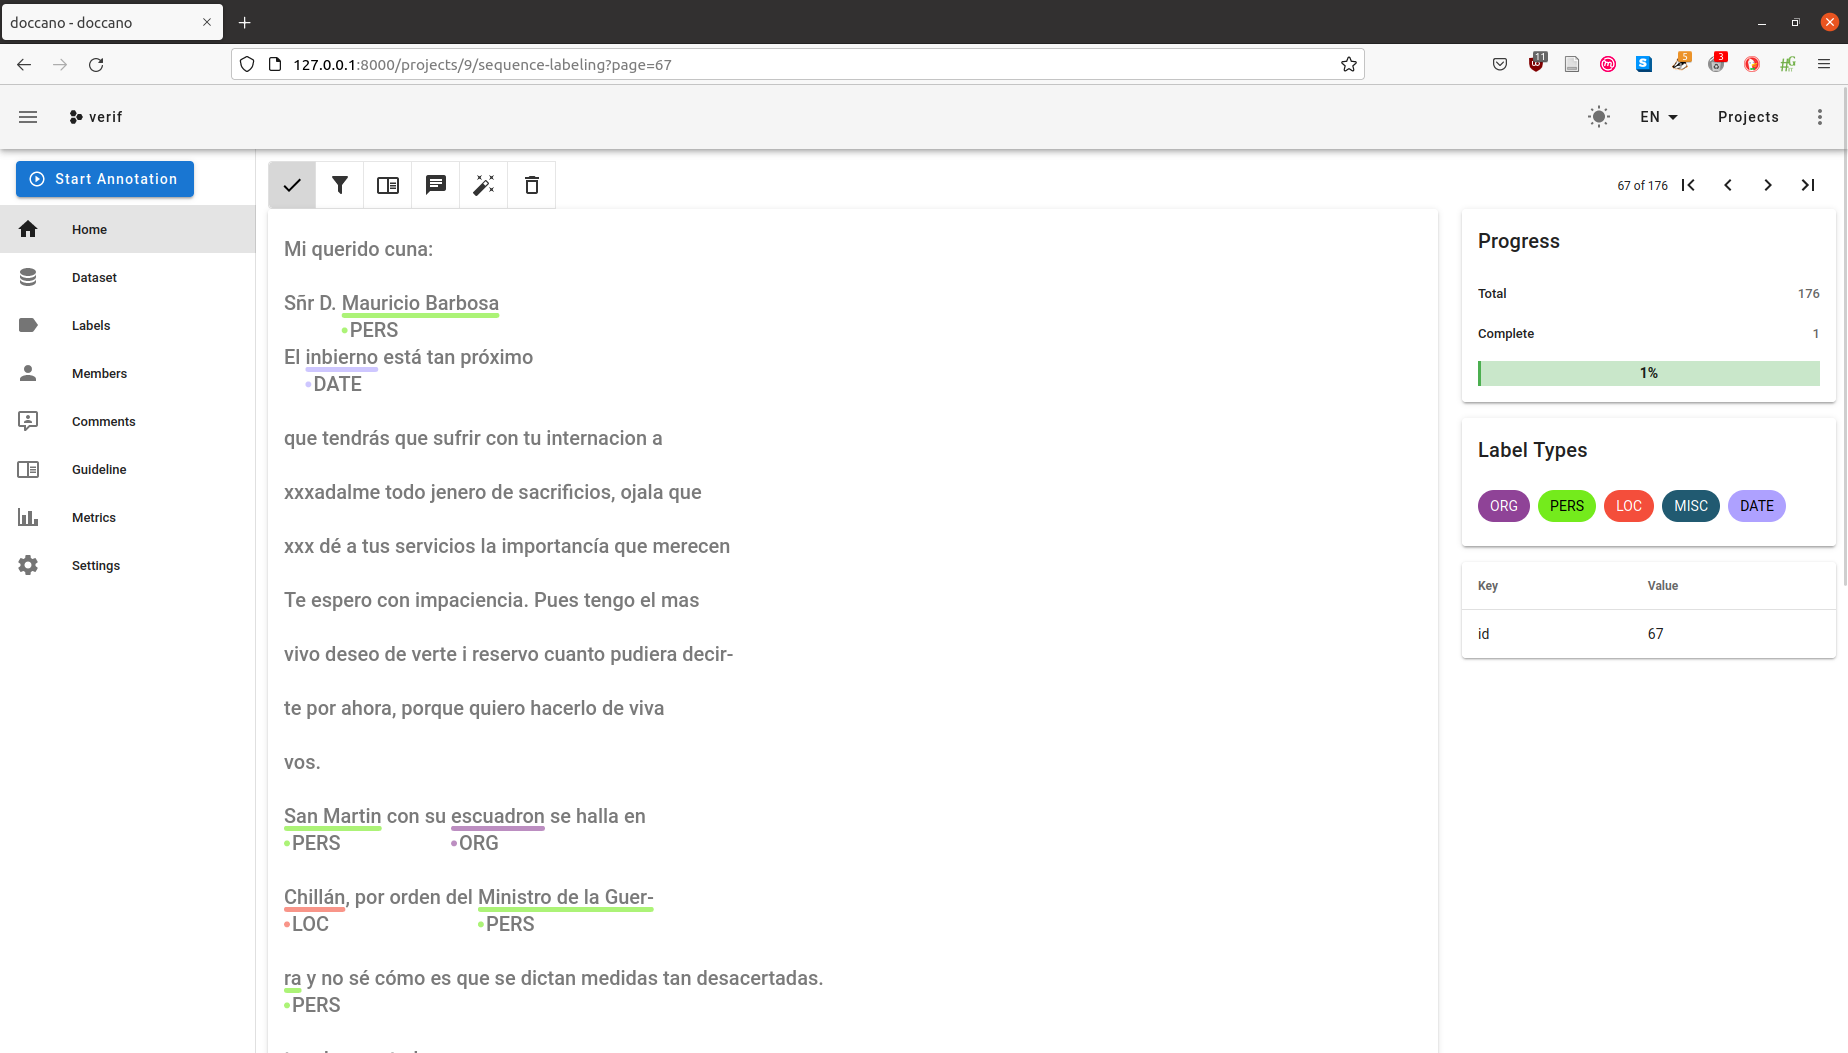
\includegraphics[width=1\textwidth]{annexes/img/doccano.png}
        \caption{Démontrastion de la plateforme Doccano}
        \label{fig:doccano}
    \end{figure}
    
    Si il est possible d'exercer une pré-annotation automatique à partir de modèle générique de NER ou d'appliquer des systèmes de règles, nous avons préféré annoter manuellement afin de s'approprier plus facilement le corpus documentaire, mais aussi les stratégies d'annotations possibles pour un corpus relativement modeste (180 documents). Pour ce faire, nous avons privilégiée la plateforme d'annotation \textit{open-source} \texttt{Doccano} pour son accessibilité et son orientation vers la librairie de \gls{tal} \gls{spacy}\footcite[Cette plateforme a été programmé avec le langage python et le \textit{framework} Django.][]{nakayamaDoccano2022}. Cet outil multifonctions d'annotation de données a été installé en local à partir du système Docker. À l'image de la figure \ref{fig:doccano}, les différentes séquences de caractères sont étiquetées de manière exclusive, c'est-à-dire à dire qu'une entité ne peut pas appartenir à une entité plus large afin d'éviter les futures confusions possibles. Cette définition a déjà été faite au sein de la conférence CoNLL 2003 où les chercheurs Erik F. Tjong Kim Sang et Fien de Meuder considéraient les entités nommées comme \enquote{non-récursive} et \enquote{\textit{non-overlapping}}\footcite{sangIntroductionCoNLL2003Shared2003}.
    
    À l'heure actuelle, \texttt{Doccano} limite l'exportation au format JSONL (pour JSON Lines), c'est-à-dire un fichier JSON dont la structuration est décomposée en plusieurs lignes. Si ce n'est pas le plus courant contrairement au format CoNLL ou autres, il permet d'obtenir une annotation simple, lisible, sans marquage et ainsi sans dissection des entités.
    
    Les schèmes IOB\footnote{I : Inside (token à l'intérieur), O: Output (token à l'extérieur), B: Beginning (token au début de l'entité). Le schème standard du format CoNLL}, BIOES\footnote{B: Beginning (début de l'entité), I : Inside (token à l'intérieur), O: Output (token à l'extérieur), E: Ending (token de fin de l'entité), S: Single element (entité consituée d'un seul token)}, BILOU\footnote{B: Beginning (token au début de l'entité), I : Inside (token à l'intérieur), L: Last (token de fin), O: Output (token à l'extérieur), U: Unit (entité constituée d'un seul token). Il est format de préférence utilisé par SpaCy.} pour les plus connus ont pour fonction d'offrir ce que l'on appelle une analyse syntaxique de surface. Le choix n'est pas anodin, car il peut avoir une incidence à la fois sur l'interopérabilité des données, mais aussi sur les performances du modèles\footcite{alshammariImpactUsingDifferent2021}. Nous avons choisi de laisser les annotations sans ce pré-marquage afin de conserver une facilité d'interagir avec les données, mais aussi d'éviter un impact négatif sur l'entraînement de notre modèle.
	
	\subsection{Produire un modèle appliquée à la reconnaissance des entités nommées}
	
	La généralisation du \textit{deep learning} a permis à l'indexation \gls{ren} des documents historiques de faire bondir les scores (\gls{f1}) de 10 à 20\%\footcite{ehrmannNamedEntityRecognition2021}. Avec les innovations entourant les architectures encodeurs-décodeurs, cette augmentation des résultats est encore plus probante sur la reconnaissance des entités nommées au sein des documents historiques au delà des problèmes qu'ils impliquent, et ce malgré un corpus pouvant être rudimentaire (50 documents annotés)\footcite{abadieBenchmarkNamedEntity2022}.
	
	\subsubsection{Entraîner un modèle NER en validation croisée}
	
	Au regard de ces observations, nous nous sommes essayé au développement d'un modèle \gls{ren} à partir du modèle pré-entraîné BETO que nous avons vu précédemment\footcite{caneteSpanishPreTrainedBERT2020}. Ce pré-entraînement permet la modification du modèle initiale afin de lui donner une tâche précise grâce au \textit{finetuning} et ainsi modifier les poids au sein de l'architecture neuronale selon nos besoins. Pour ce faire, de nombreuses librairies python permettent de mettre en œuvre ce type d'entraînement à partir de modèles pré-entraînés \textit{Transformers}. \gls{spacy} et \texttt{HuggingFace} sont sans doute à l'heure actuelle les plus populaires, car elles offrent des solutions \gls{tal} clés en main, ergonomiques et accessibles. Si elles sont par nature restrictives, elles restent suffisantes à l'ambition du projet qui ne nécessite pas une refonte neuronale totale contrairement à des projets amplement plus complexes. Nous avons privilégié l'utilisation de la librairie \gls{spacy} en raison de la galaxie de solutions \textit{softwares} qui l'entourent, le maintien d'une documentation exhaustive et extrêmement pédagogique avec la possibilité d'utiliser les modèles \textit{Transformers} grâce à la mise en place d'une \textit{pipeline} pour l'utilisation des modèles originalement disponibles au sein de la librairie \texttt{HuggingFace}\footcite{SpacytransformersUsePretrained2022}.
	
	Au préalable, il est à noter que le processus d'apprentissage de modèles \textit{Transformers} nécessite une grande puissance de calcul. Dans un premier temps, nous avons souhaité utilisé la plateforme Google Colab\footnote{\textit{Google Colab}, \url{https://colab.research.google.com/}, consulté le 04/09/2022.} mettant à disposition l'utilisation de \gls{gpu} par l'intermédiaire de leurs serveurs. Par la suite, nous avons utilisé un \gls{gpu} personnel pouvant avoir eu une incidence sur les résultats du modèles\footnote{Nvidia RTX 3080, CUDA 11.3, cuDNN}.
	
	\begin{figure}[h!]
	    \centering
	    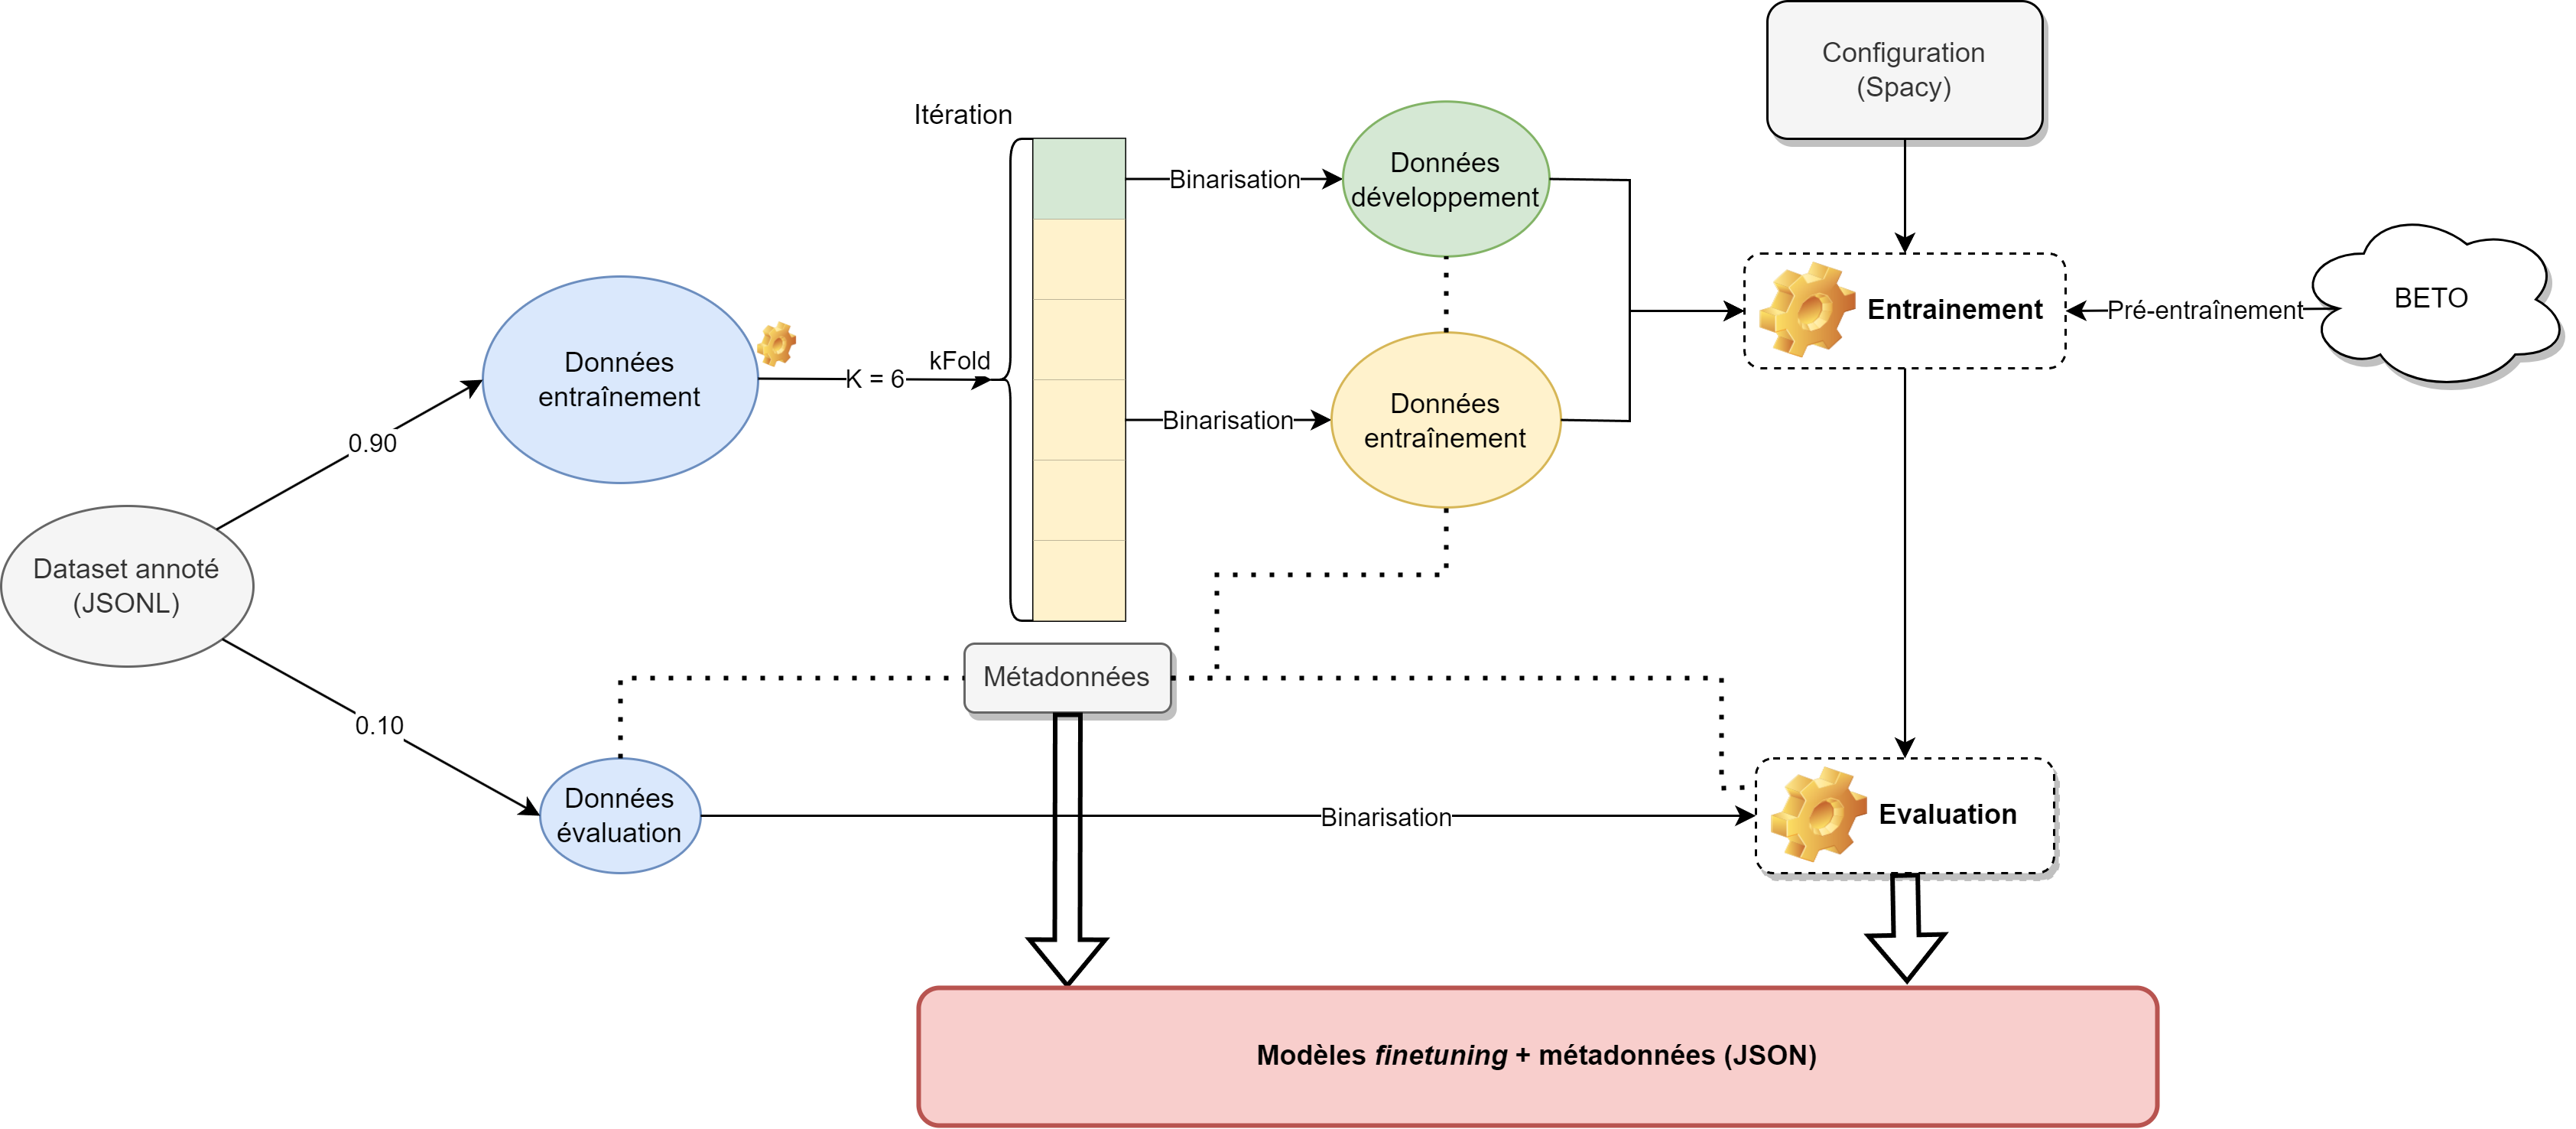
\includegraphics[width=1\textwidth]{annexes/schema/NER_training.png}
	    \caption{Schéma du processus d'entraînement d'un modèle NER en validation croisée\protect\footnotemark}
	    \label{fig:ner_cross}
	\end{figure}
	\footnotetext{\cite{humeauEntrainementAnnotationsNER2022}}
	
	Afin de mettre en oeuvre ce processus d'entraînement, nous sommes aidés de la librairie \texttt{scikit-learn} mettant à disposition un grand nombre d'outils appliqués au \textit{machine learning}\footcite{ScikitlearnScikitlearn2022}. Plus précisément, le processus s'appuie sur la séparation des données en plusieurs dépôts utilisable au cours de l'entraînement (un jeu d'entraînement et un jeu d'évaluation) afin d'offrir des jeux avec le moindre biais humain. 
	
	Dans un second temps, nous pouvons observer au sein de la figure \ref{fig:ner_cross} la présence d'une itération autour de \textit{kFold}. Cet élément correspond à la mise en place d'un procédé de validation croisée. Cette méthode K-fold, permet de tester et améliorer les performances d’un modèle prédictif en exploitant l'ensemble de notre jeu de données d'entraînement, en constituant des \textit{samples} ($\kappa$) de données partagées pour l'entraînement et sa validation. Cet technique d'apprentissage permet de maximiser le potentiel du jeu original en le prenant dans son intégralité, particulièrement quand celui-ci est restreint\footcite{perssonEffectExcludingOut2017}. Les données d'évaluation restent les mêmes tout au long du processus afin de fournir des données tests stables et ainsi fournir une évaluation fiable.
	
	Chaque itération détermine un set de données d'entraînement et de validation (qui ne pourra donc plus l'être par la suite) qui sont alors binarisées pour être exploitables par le \gls{cli} de \gls{spacy}. Le programme va effectué une première modélisation avec le modèle pré-entrainé BETO avant d'incorporer les données d'entraînement au sein de l'apprentissage. Chaque étape se conclut par un processus d'évaluation qui détermine ses performances à chaque \textit{epoch} à partir des données d'évaluation. Une fois le meilleur modèle estimé, celui-ci est évalué à partir des données tests dont les résultats sont associés à un fichier \gls{json}.
	
	\begin{figure}[h!]
	    \centering
	    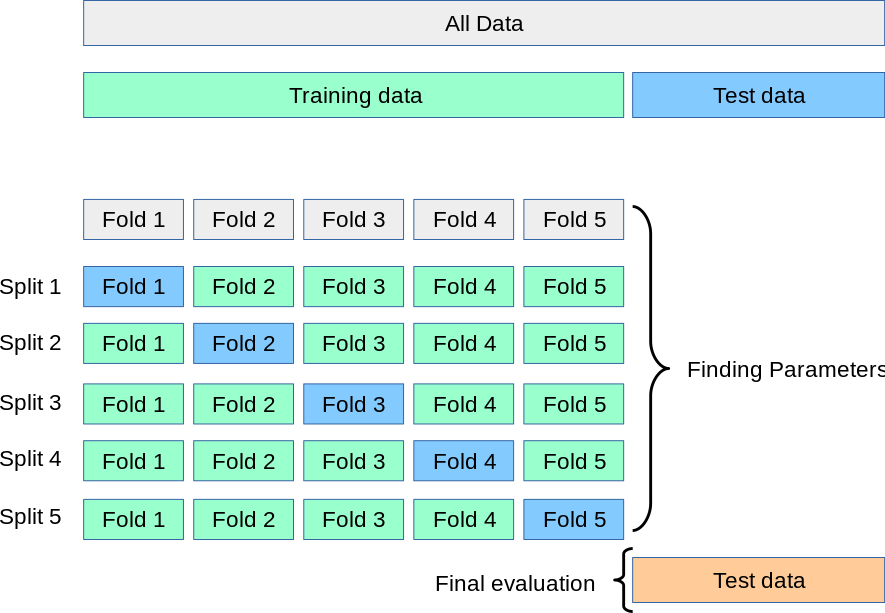
\includegraphics[width=0.5\textwidth]{annexes/schema/cross_validation.png}
	    \caption{Explication du système de validation croisée à partir de la méthode K-fold -- \copyright scikit-learn}
	    \label{fig:cross validation}
	\end{figure}
	
	\subsubsection{Interprétation des résultats et améliorations possibles}
	
	À partir de ces résultats, nous pouvons comparer les différents modèles afin de déterminer le plus performant d'entre eux\footnote{L'ensemble des données sont consultables au sein de l'annexe F.}. Cette phase d'évaluation consiste à estimer la capacité du modèle à sélectionner la bonne chaîne de caractères et d'attribuer à cette chaîne le référentiel adéquat. Pour cela, trois mesures basées sur la matrice de confusion sont considérées les plus pertinentes par la communauté scientifique: \gls{ACC}, \gls{rappel}, \gls{f1}\footcite{liSurveyDeepLearning2020}. Elles permettent d'avoir une perception globale du modèle en évaluant le taux de bonnes réponses sur les supposées entités repérées. Le score \gls{f1} décrit une valeur globale en conciliant les deux mesures\footnote{D'autres métriques plus complexes existent aussi pour l'évaluation des modèles \gls{ren} tel que la mesure SER, mais nous avons conserver les mesures proposées par \texttt{spaCy}. \cite{ehrmannNamedEntityRecognition2021}}.
	
	\begin{figure}[h!]
	    \centering
	    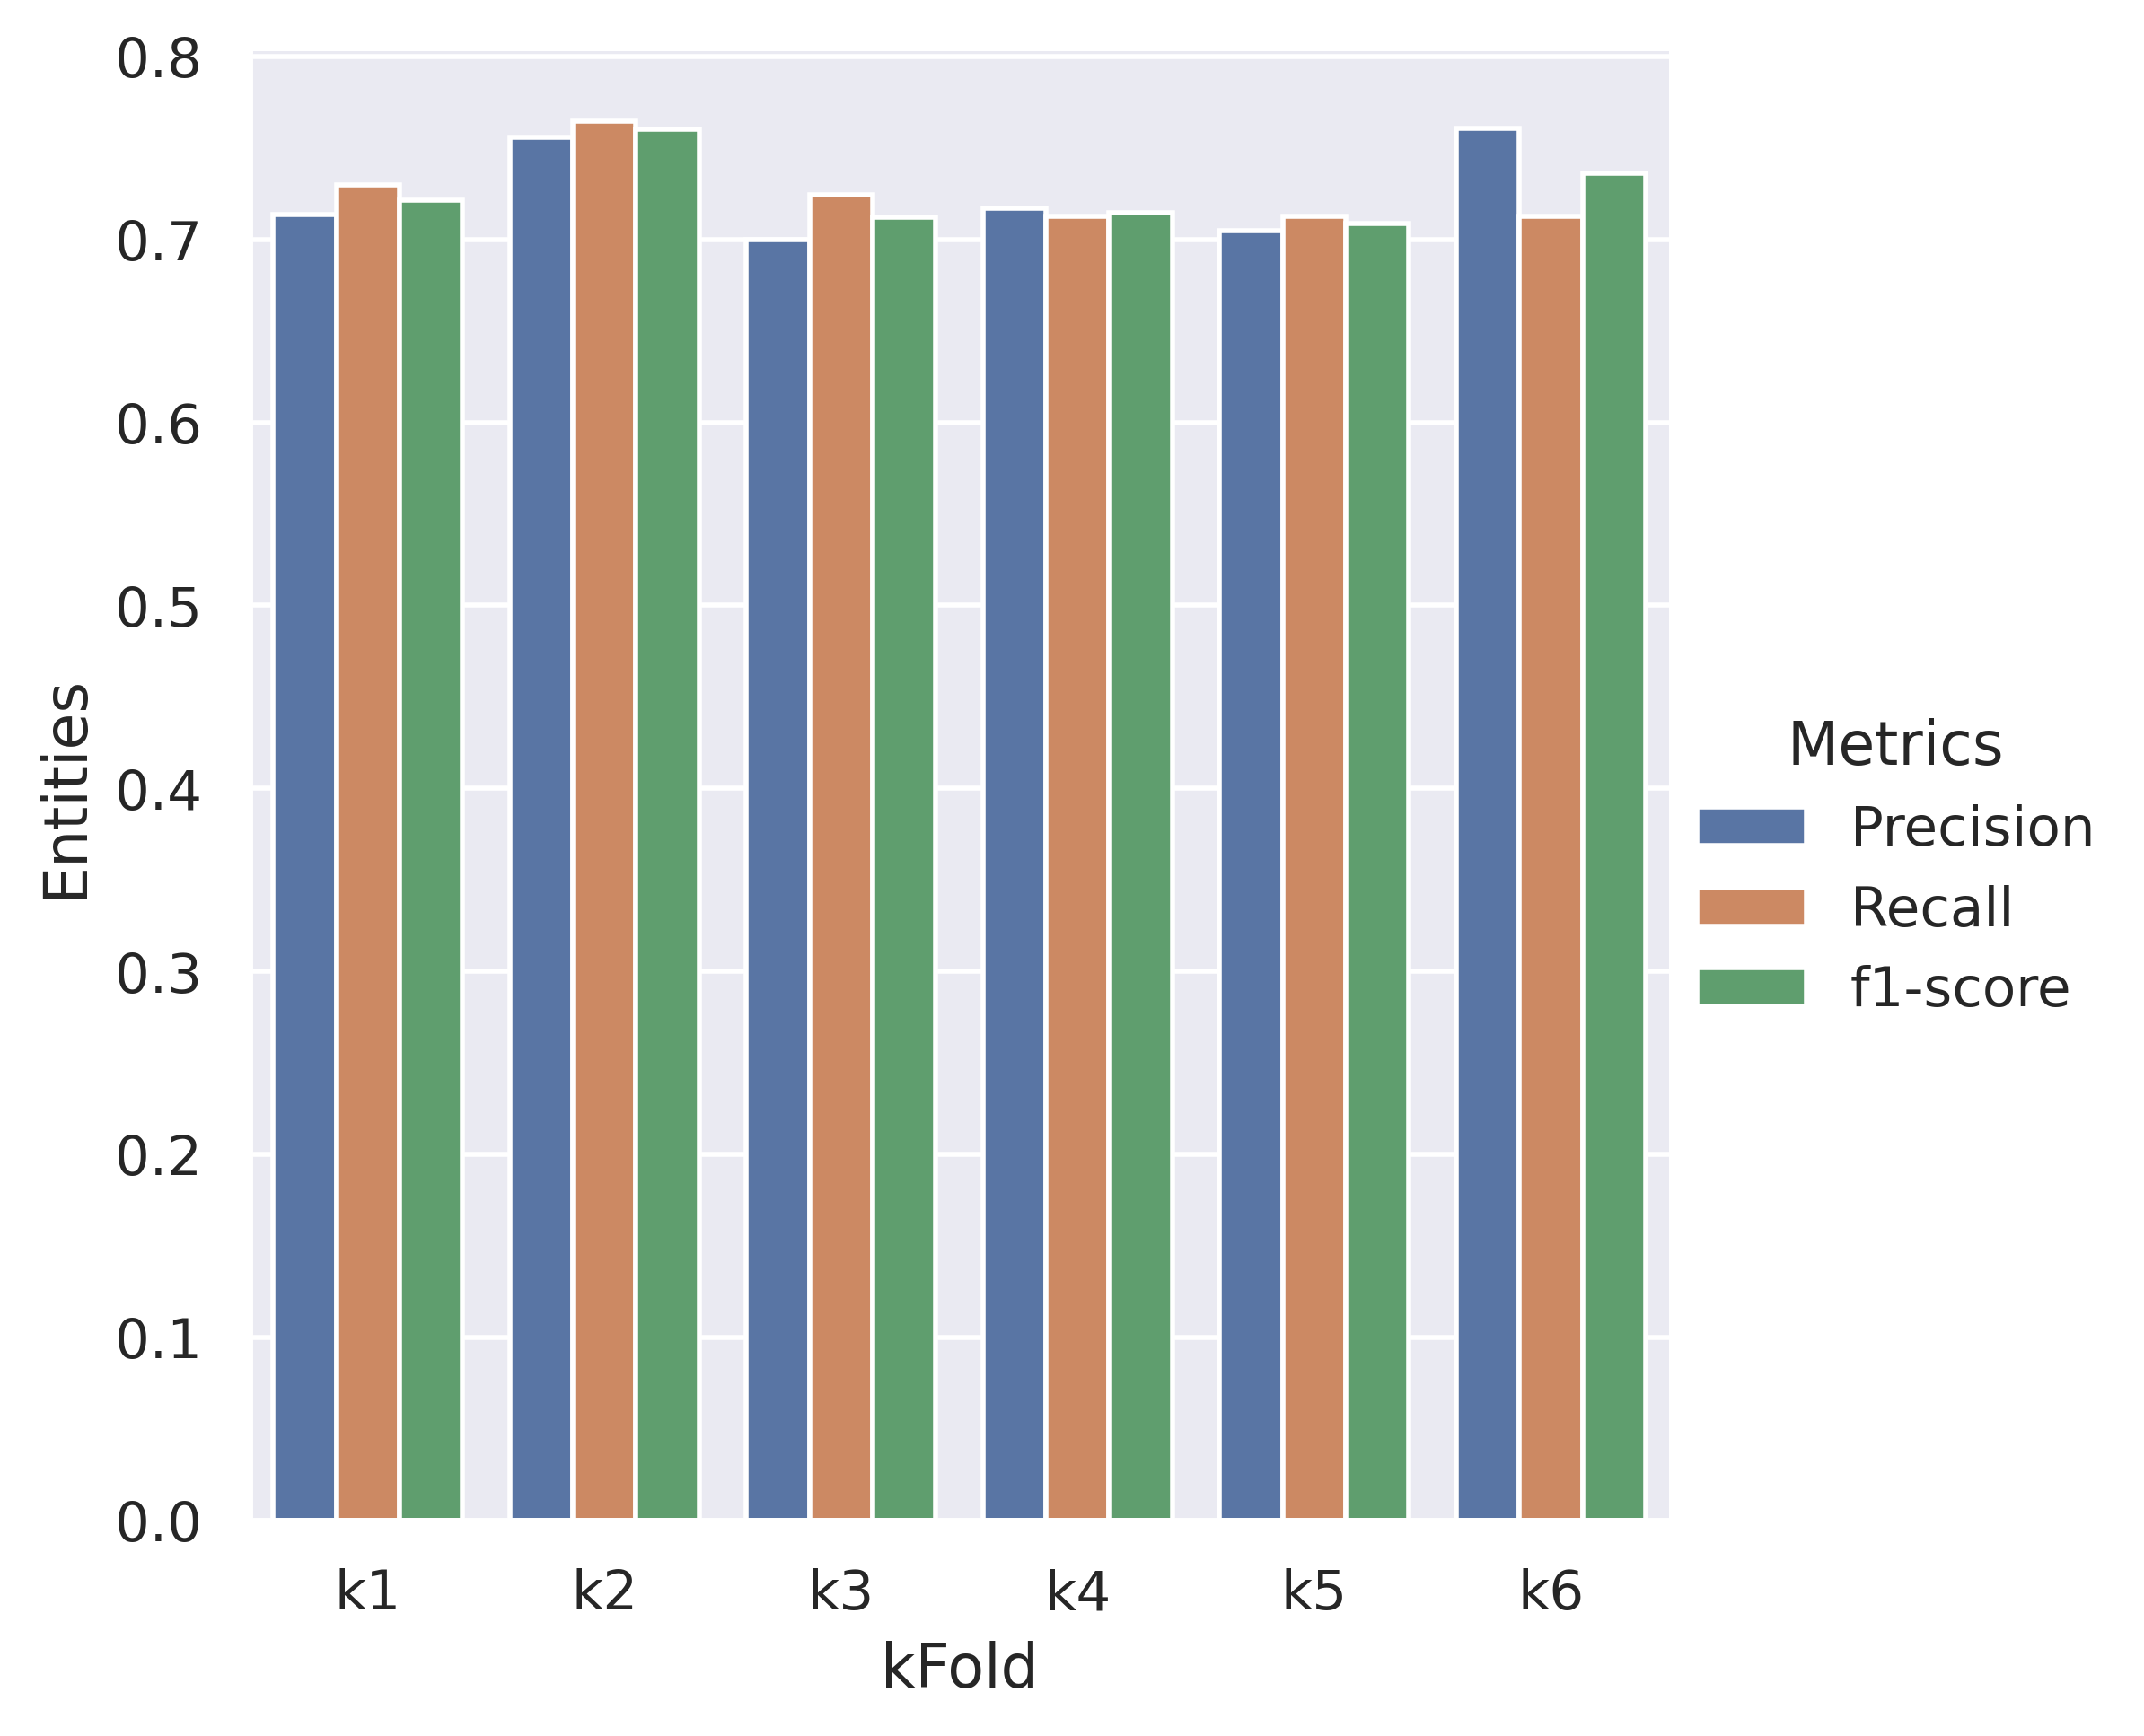
\includegraphics[width=0.4\textwidth]{annexes/graph/ent_glob.png}
	    \caption{Résultats globaux par $\kappa$ selon les trois mesures principales}
	    \label{fig:ner_global}
	\end{figure}
	
	Selon les mesures présentées, les différents modèles ont été analysés selon leurs performances comme nous pouvons l'observer au sein de la figure \ref{fig:ner_global}. Au regard des données qui ont été évaluées, deux modèles sont apparus comme les plus solides: le modèle $\kappa_2$ et le modèle $\kappa_6$. À première vue, le modèle $\kappa_2$ apparaît comme le plus satisfaisant, avec un taux de surpositivité plus faible comme le montre la valeur de \gls{rappel}.
	À la suite d'une comparaison plus approfondie entre les deux modèles sélectionnés, nous avons pu observer une lacune générale sur les entités MISC qui peut s'expliquer par la forte diversité de celle-ci. Toutefois, certaines entités semblent plus accessibles que d'autres à l'image des navires qui sont facilement identifiables\footnote{Voir l'annexe G.}. En revanche, on observe une légère supériorité du modèle $\kappa_2$ concernant les entités de type LOC, PERS et plus légèrement ORG. Sur l'ensemble, le modèle $\kappa_2$ semble produire plus de bruit dans la reconnaissance des données, ce qui s'observe avec le fort contraste entre le taux de précision et le taux de rappel. 
	
	Face à ce constat, nous avons privilégié l'emploi du modèle $\kappa_2$ qui semblent présenter des performances globales plus pertinentes dans le cadre du projet, avec une attention particulière sur les entités LOC et PERS estimés les plus indispensables à l'édition en vue de l'enrichissement des données. Sans être excellente, les performances du modèle \gls{ren} peuvent être classé comme positives si on le compare à d'autres expérimentations, plus particulièrement en raison de la faible quantité de données ajoutées\footcite[p.~105-109]{scheithauerReconnaissanceEntitesNommees2021}. De plus le réseau neuronal semble avoir rapidement assimilé l'entité DATE qui est souvent présentée de manière structurée. En revanche, on peut remarquer une forte fébrilité sur la reconnaissance de certains notamment \enquote{Usted} pouvant être associé à la fois au référentiel LOC, MISC ou ORG. De même, il semble parfois amalgamer certaines entités avec leurs prépositions.
	
	Afin de perfectionner ce modèle, deux solutions possibles ont été décrites afin de faire face aux problèmes constatés. La première est de spécifier plus en détail les entités MISC qui sont trop généralistes. L'autre axe d'amélioration est ce que l'on appelle la désambiguïsation et la relation des entités nommées (\textit{entity linking} en anglais) qui n'ont pas pu être mises en place pour l'instant faute de temps\footcite{ehrmannNamedEntityRecognition2021}. Le modèle doit être capable de reconnaître la référence d'un mot au-delà de sa polysémie. Par exemple, \enquote{Arauco} peut signifier à la fois une ville et une administration régionale. En général, cette désambiguïsation s'appuie sur l'entraînement d'un modèle à partir d'une base de connaissance extérieure en identifiant les éléments polysémiques\footcite{bunescuUsingEncyclopedicKnowledge2006}. Cette stratégie est appelée \textit{entity linking} et elle permet l'identification  du mot, par une approche vectorielle ou syntaxique, en l'alignant au près de grandes bases de connaissances accessibles \textit{via} le web sémantique\footcite{morenoApprendreRepresentationsJointes2017}.
	
	\begin{figure}[H]
         \centering
         \begin{subfigure}[b]{0.4\textwidth}
             \centering
             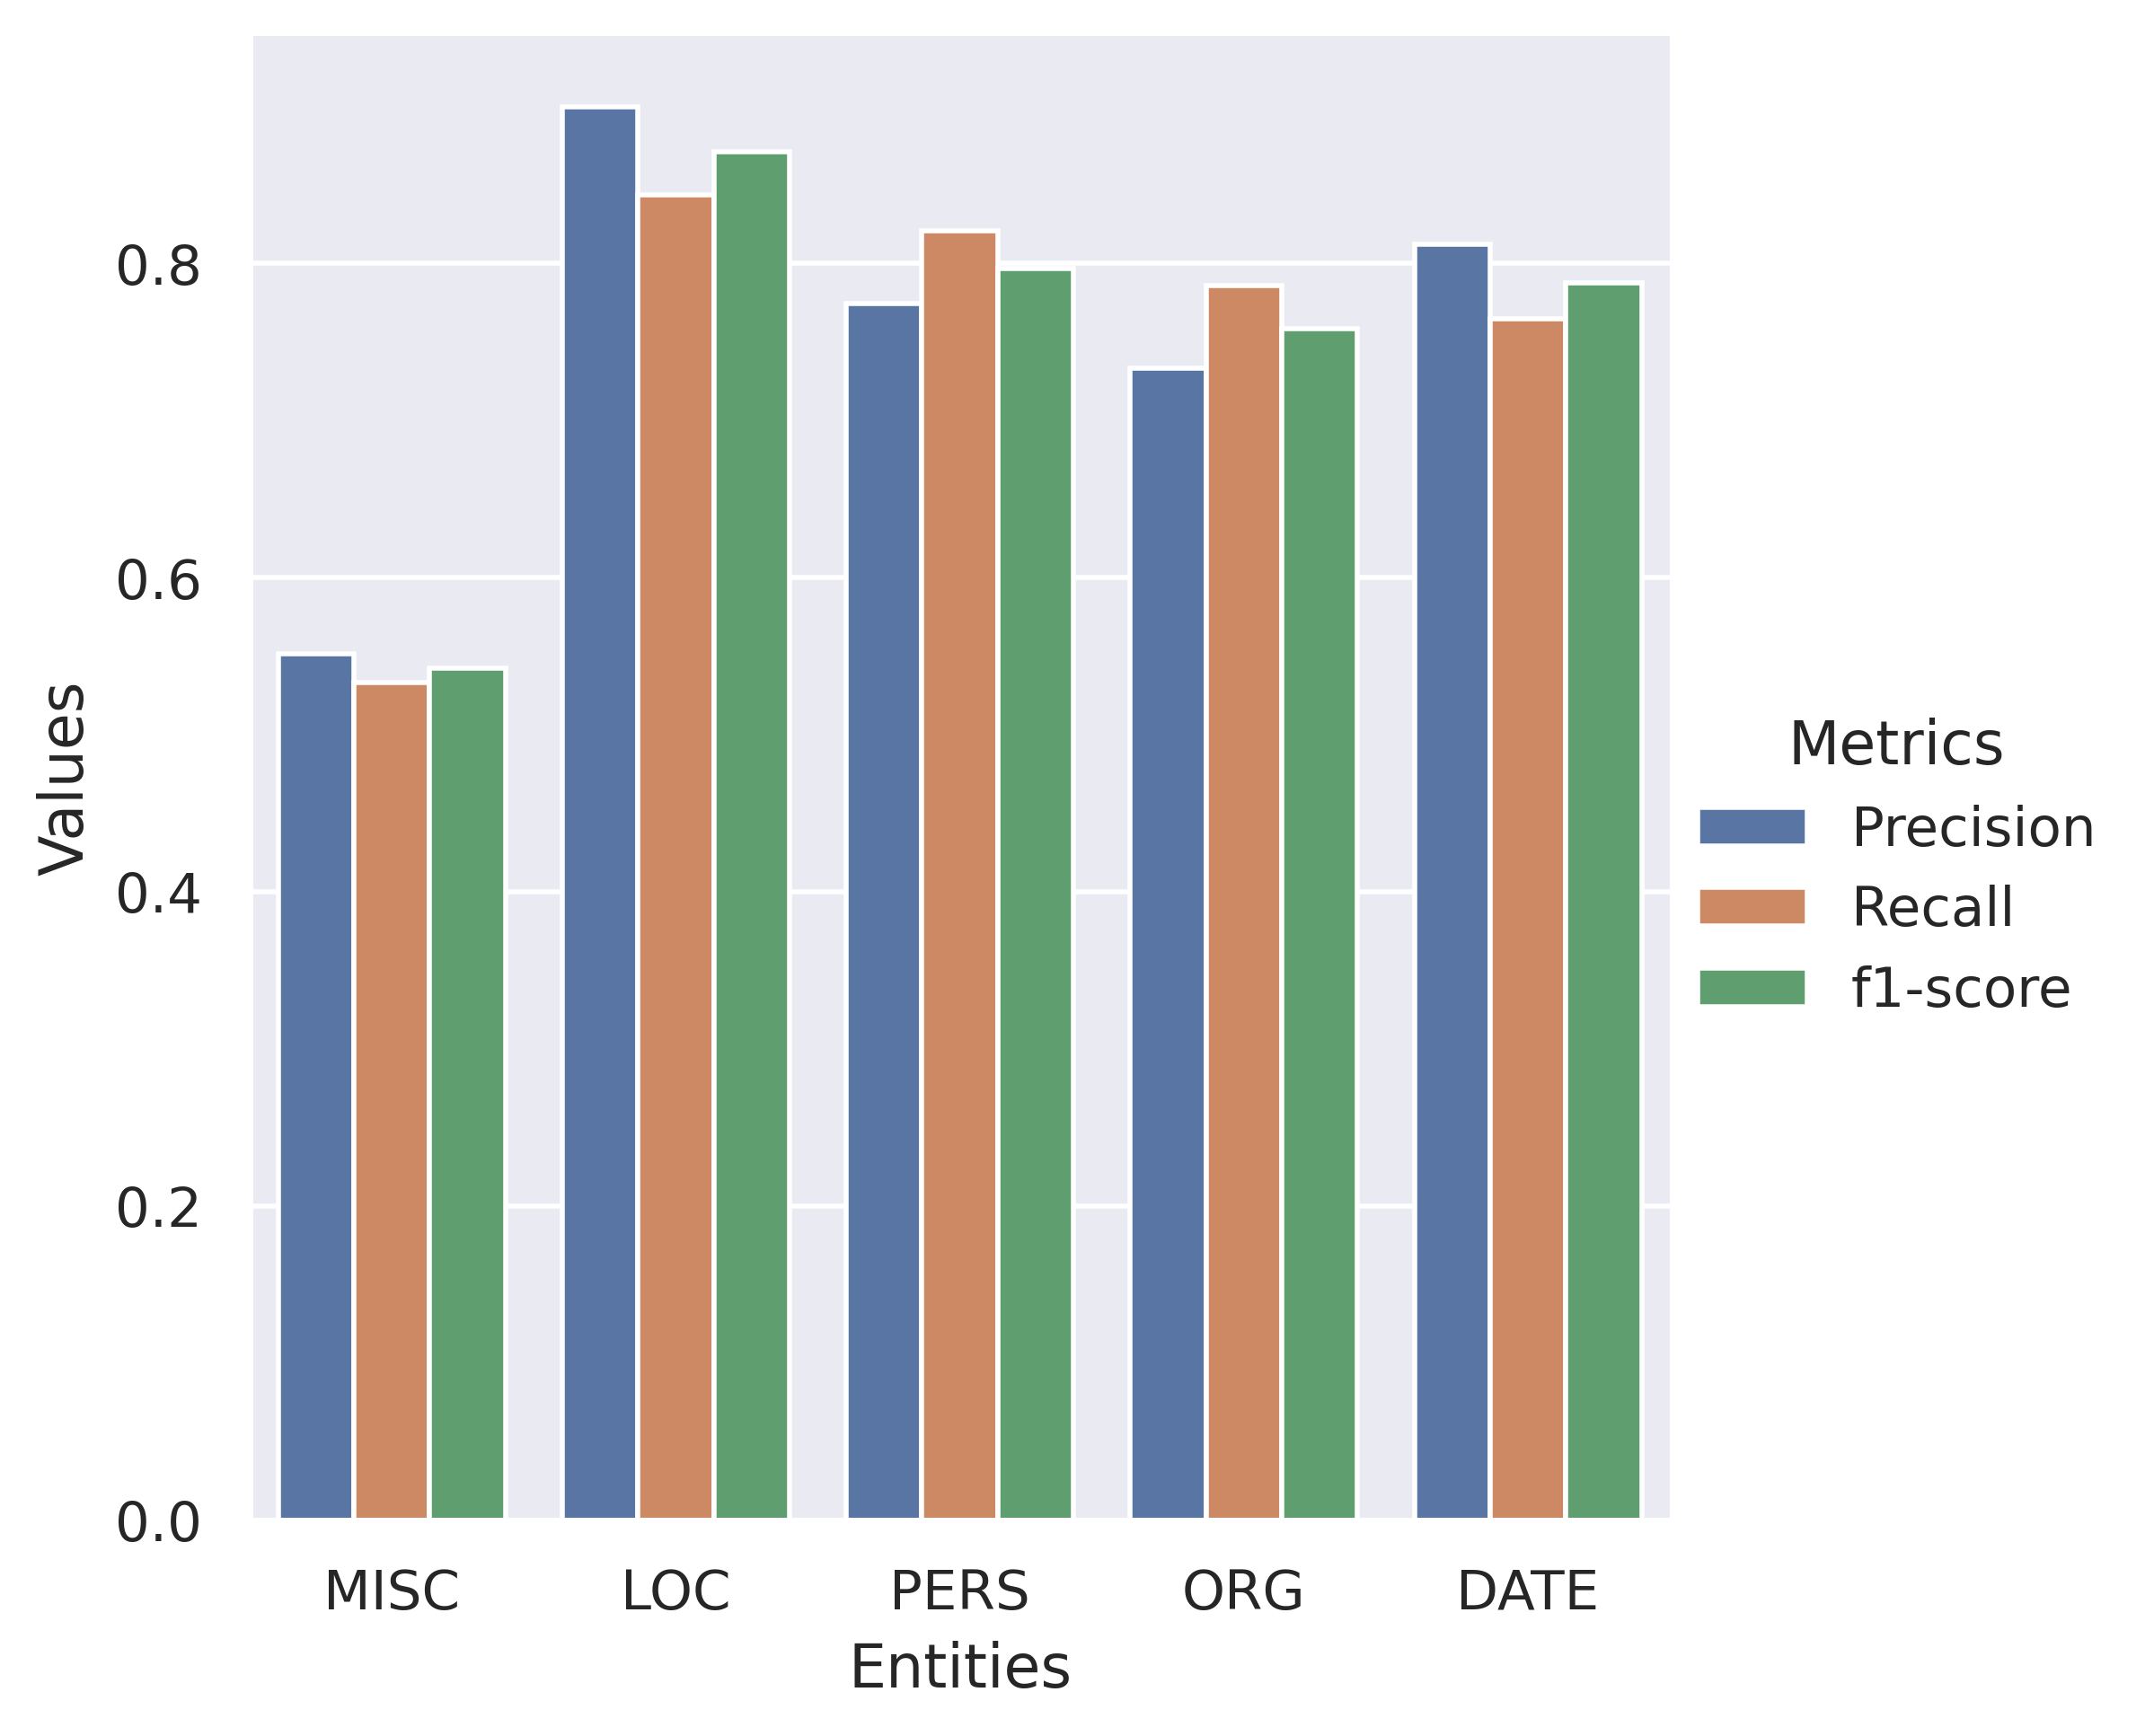
\includegraphics[width=\textwidth]{annexes/graph/k2.png}
             \caption{$\kappa_2$}
             \label{fig:k2}
         \end{subfigure}
         \hfill
         \begin{subfigure}[b]{0.4\textwidth}
             \centering
             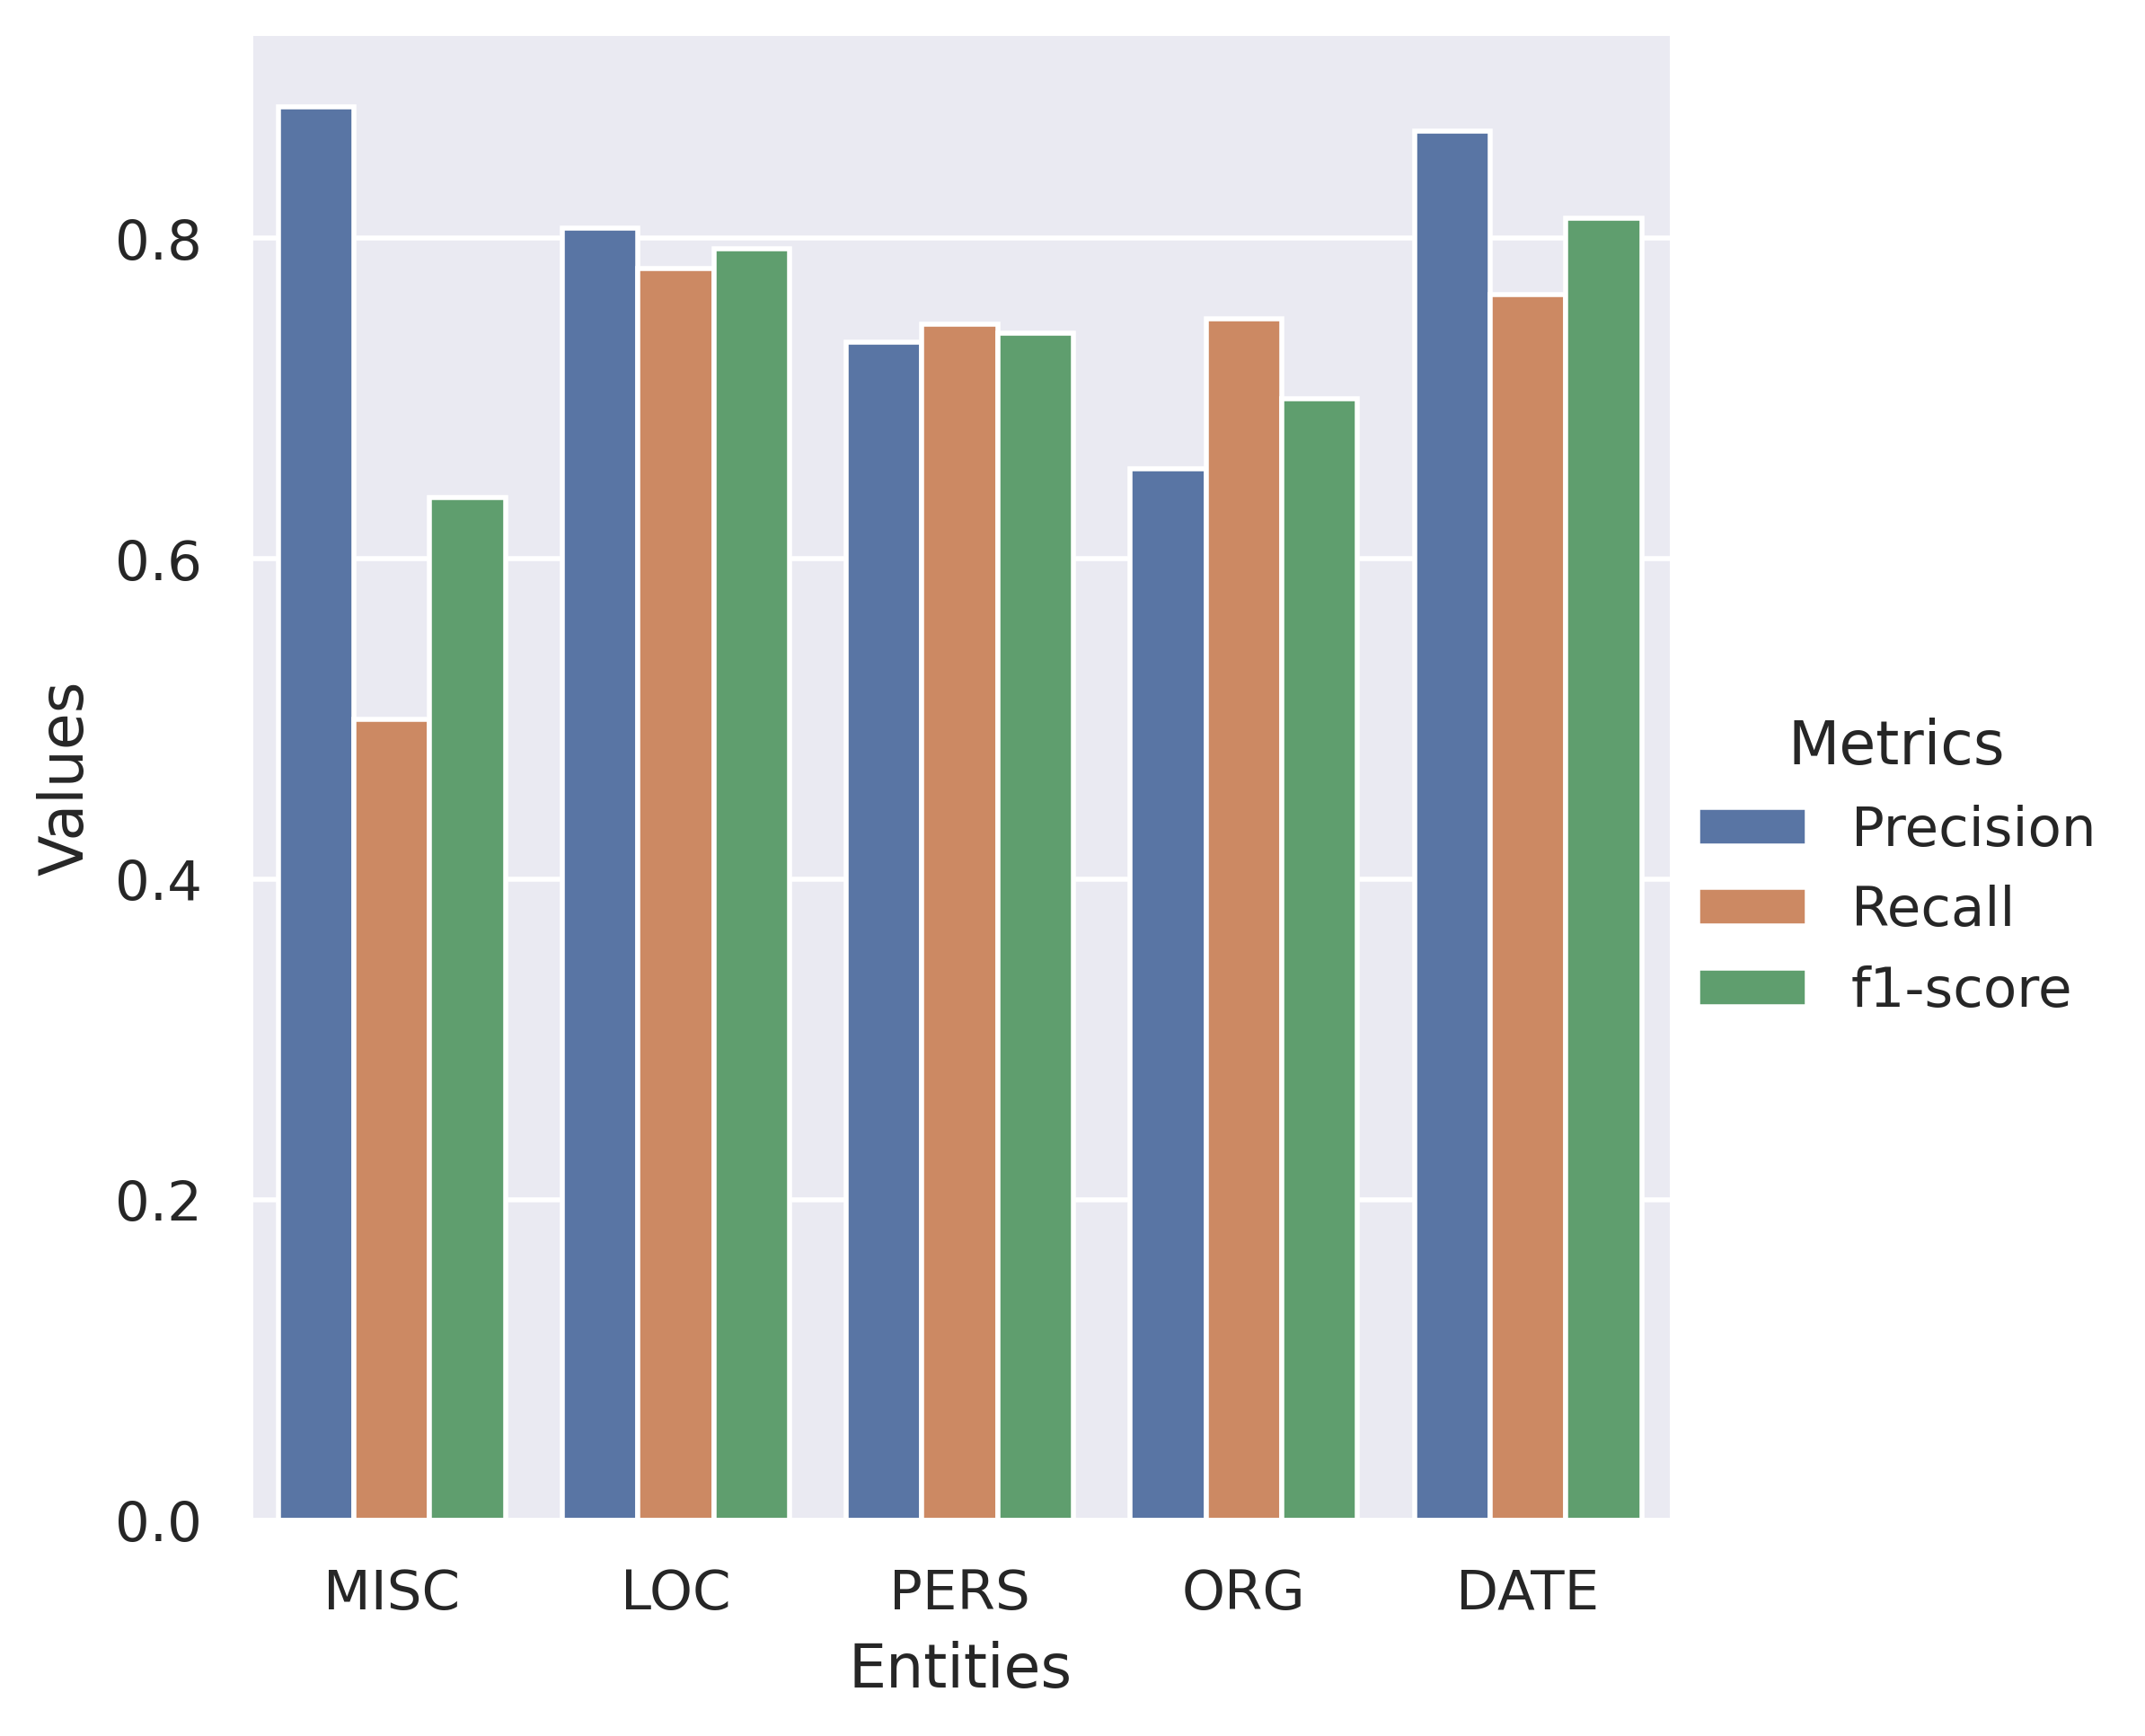
\includegraphics[width=\textwidth]{annexes/graph/k6.png}
             \caption{$\kappa_6$}
             \label{fig:k6}
         \end{subfigure}
         \caption{Résultats détaillés par entité}
        \label{fig:ner_results}
    \end{figure}
    
    \begin{table}[H]
    \centering
    \begin{tabular}{c|r|r|r|}
    \cline{2-4}
    \textbf{}                              & \multicolumn{1}{c|}{\textbf{Precision}} & \multicolumn{1}{c|}{\textbf{Rappel}} & \multicolumn{1}{c|}{\textbf{F1-score}} \\ \hline
    \multicolumn{1}{|c|}{\textbf{Général}} & 0.7556                                  & 0.7643                               & 0.7600                                 \\ \hline
    \multicolumn{1}{|c|}{\textbf{MISC}}    & 0.5517                                  & 0.5333                               & 0.5423                                 \\ \hline
    \multicolumn{1}{|c|}{\textbf{LOC}}     & 0.9000                                  & 0.8437                               & 0.8709                                 \\ \hline
    \multicolumn{1}{|c|}{\textbf{DATE}}    & 0.8125                                  & 0.7647                               & 0.7878                                 \\ \hline
    \multicolumn{1}{|c|}{\textbf{PERS}}    & 0.7746                                  & 0.8208                               & 0.7971                                 \\ \hline
    \multicolumn{1}{|c|}{\textbf{ORG}}     & 0.7333                                  & 0.7857                               & 0.7586                                 \\ \hline
    \end{tabular}
    \caption{Évaluation des performances du modèle $\kappa_2$}
    \label{tab:k2_benchmark}
    \end{table}
	
	
	\section{Indexer, enrichir et exploiter les données}
	
	La reconnaissance des entités nommées offre une double opportunité. Elle permet dans un premier temps d'indexer l'ensemble des entités et ainsi faciliter l'accès à cette donnée pour l'utilisateur ou l'utilisatrice. L'autre aspect est la capacité de renforcer les mécanismes d'enrichissement au cours du processus éditorial. Cet enrichissement est en général un exercice conséquent et pour autant nécessaire dans la constitution d'un apparat critique\footcite{campsOuVaPhilologie2018}.
	 
	 Dans cette perspective nous allons observer la mise en place d'un processus d'indexation et d'enrichissement automatique grâce à l'aide de l'\textit{open data} et les problématiques que ce procédé impose.
	
	\subsection{Indexer les entités nommées au sein d'une édition numérique TEI}
	
	La première difficulté qui a été rencontré dans l'application d'un schéma d'indexation a été simplement d'appliquer la reconnaissance au sein d'un fichier structuré et de conserver cette structuration, dans notre cas \gls{xml} et de l'encodage \gls{tei}. Au retour des campagnes d'annotations ESTER, Solenn Le Pevedic et Denis Maurel approuvent la capacité de l'encodage à manipuler les entités nommées en permettant une normalisation des éléments descriptifs\footcite{lepevedicRetourAnnotationsEntites2016a}. Au sein de cet article, les auteurs vont émettre de premières recommandations sur le balisage de ces entités en fonction de leur référentiel, et les attributs adéquats, en reprenant le guide Quaero.
	
	\begin{figure}[h!]
	    \centering
	    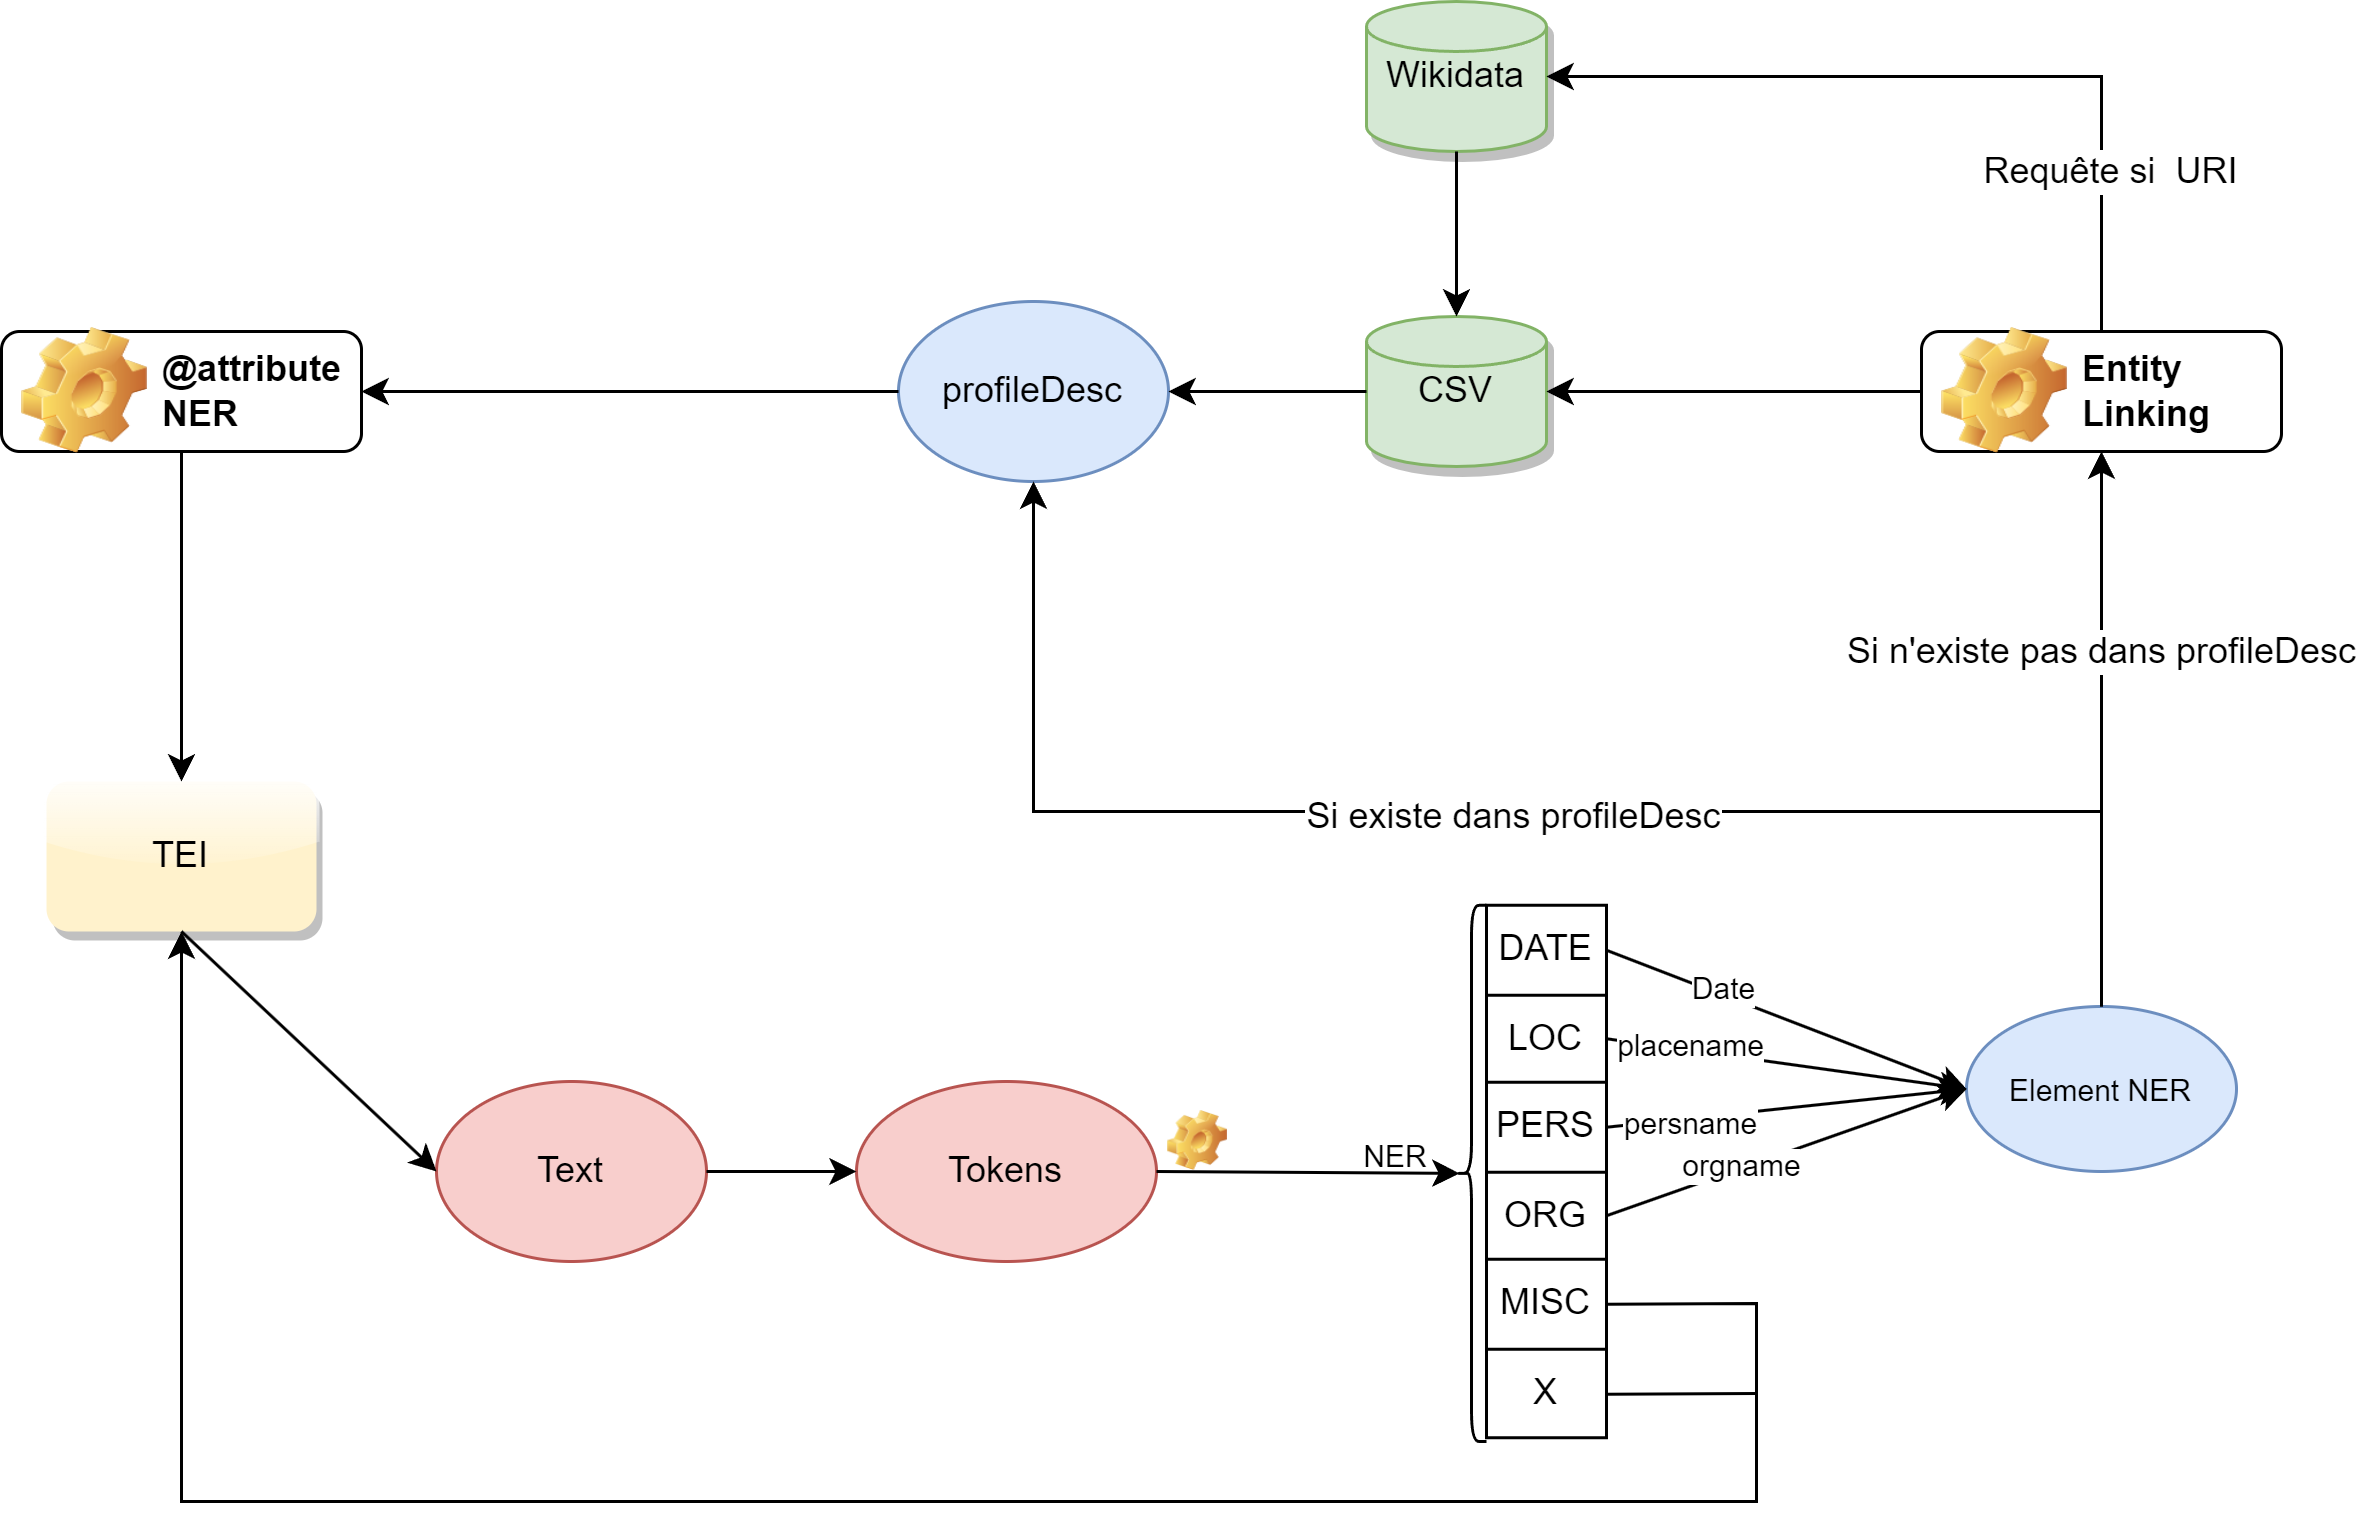
\includegraphics[width=0.8\textwidth]{annexes/schema/ner_index.png}
	    \caption{Système d'indexation des entités nommées au sein d'un fichier XML-TEI}
	    \label{fig:ner_index}
	\end{figure}
	
	Pour manipuler nos fichiers XML-TEI déjà existants, nous nous sommes appuyés sur la librairie \texttt{StandoffConverter} développée récemment par David Lassner\footcite{lassnerStandoffconverter2021}. L'utilisation de son \gls{API} permet le balisage des entités détectées par le modèle développé\footcite[Le script est visible au chemin suivant : TEI\_tranformation/src/enrichment/nlp.py \textit{in}][]{humeauTeiTransformation2022}. Pour ce faire, la classe StandoffConverter va analyser l'ensemble du \balise{text}, le tokeniser et repérer son référentiel au sein des catégories définies par le modèle \gls{ren}. Cette librairie a permis de faciliter ce travail d'extraction et les problèmes sous-jacents en limitant l'impact de la structuration \gls{xml} en permettant de convertir certains éléments sous la syntaxe \gls{regex}, par exemple : \balise{lb} pour \textbackslash n.
	
	Pour chaque entité, nous avons remis les recommandations de balisage émises par S. Le Pevedic et D. Maurel en les simplifiant afin de permettre l'automatisation de l'indexation\footcite{lepevedicRetourAnnotationsEntites2016a}. Ainsi, l'entité DATE est balisée sous l'élément \balise{date}, LOC est balisée sous l'élément \balise{placename}, PERS est balisée sous l'élément \balise{persname} et ORG est balisé sous l'élément \balise{orgname}. À l'inverse, les tokens MISC ou sans labélisation ne sont pas référencés dans le fichier XML-TEI final.\newpar
	
	Les entités balisées sont ensuite analysées par la librairie \texttt{spaCy Fishing} afin de déterminer les possibles ambiguïtés et pouvoir les aligner au sein du web sémantique. Cette librairie a été développée par Lucas Terriel, inspiré par les travaux de Patrice Lopez sur la désambiguïsation des entités nommées et les fonctions d'\textit{entity linking}\footcite{terrielSpaCyFishing2022}. Elle est une fonctionnalité rattachable aux fonctions sommaires de \gls{spacy}, faisant la liaison entre la détection d'entités nommées et l'identification au sein d'une base de connaissances, ici \textit{Wikidata}. Si le score de l'évaluation de cette requête est supérieur à 0.8, l'\gls{uri} de l'entité (ex: Q4233309 pour Cornelio Saavedra Rodríguez) est alors conservée et enregistrée au sein de la base de données \gls{csv}, sinon un identifiant est généré si l'entité n'est pas déjà référencée au sein de la base de données.
	
	Cette chaîne d'extraction d'informations a dans le même temps été appliquée au sein du projet NER4Archives\footcite{clavaudNER4ArchivesNamedEntity2022}. Néanmoins, dans notre cas les résultats donnés par cette pratique de \textit{fishing} ont démontrés de nombreuses lacunes. Les premiers essais ont montré une réelle difficulté à déterminer et aligner la bonne entité avec un haut niveau de certitude. La gestion des abréviations n'ayant pu être pour l'instant incorporée au sein du processus de transformation, l'alignement avec la base de données \texttt{wikidata} ne peut se faire correctement.
	
	\subsection{Le web de données : SPARQL et Wikidata}
	
	L'identifiant des entités nommées permet l'accès d'un point de référence à la fois au sein de la base de données \gls{csv}, mais aussi à l'intérieur de notre encodage \gls{tei}. Au sein des éléments, cet identifiant est indiqué à l'intérieur d'un attribut \attribut{ref} le reliant directement à son élément parent présent au sein des index définis par la \gls{tei}. Pour le cas des entités LOC, celles-ci sont enregistrées au sein du \balise{settingDesc}, alors que les entités ORG et PERS sont quant à elles recensées au sein du \balise{particDesc}. Ce référencement permet de décrire plus en détail les différents éléments indexés.
	
	Comme le rappelle Simon Hengchen et al., l'effervescence du web de données a eu un réel impact auprès des secteurs culturels en donnant des points d'accès à des bases de données permettant d'enrichir considérablement leurs propres collections\footcite{hengchenExtractionEntitesNommees2015}. Une méta-étude recense justement que la recherche et l'exploration de données sont les principaux facteurs dans le choix de mettre en place ces bases de données liées\footcite{davisLinkedDataCultural2021}. La \gls{ren} sert de point d'accroche avec les données présentes au sein de web de données (\textit{linking data}). Cette notion est apparue dans les années 1990 sous l'égide de Tim Berner-Lee qui la définit comme un espace d'échange de documents permettant d'accéder à leurs contenus et effectuer des raisonnements\footcite{berners-leeSemanticWeb2001}. Les contenus sont communément appelés des ressources qui doivent être organisées de manière structurée afin d'être intelligible, souvent à partir de la syntaxe \gls{rdf}.  La relation sémantique entre les ressources est possible sous la forme de \enquote{triplet} : Sujet (ressource principale) -- Prédicat (relation) -- Objet (ressource secondaire). La représentation \gls{rdf} va s'appuyer sur un ensemble de classes (Sujets) et de propriétés intrinsèques permettant d'être reliée entre elles.
	
	\begin{figure}[H]
	\centering
    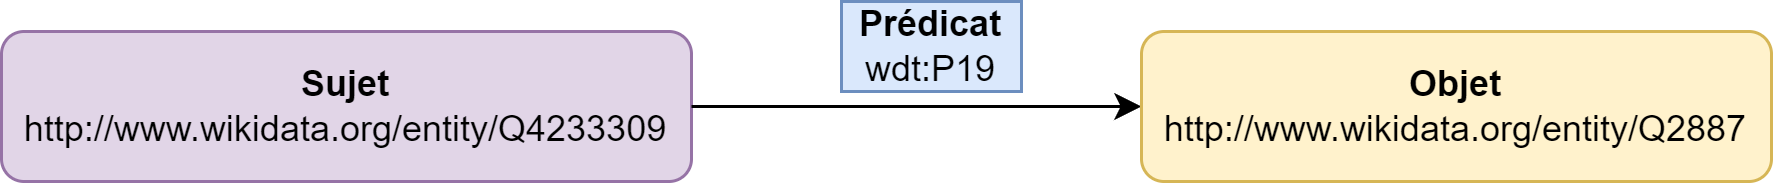
\includegraphics[width=0.7\textwidth]{annexes/schema/triplet.png}
    \begin{minted}[fontsize=\footnotesize]{xml}
          <?xml version="1.0"?>
          <rdf:RDF xmlns:wdt="http://www.wikidata.org/prop/direct/" xmlns:schema="http://schema.org/">
            <rdf:Description rdf:about="http://www.wikidata.org/entity/Q4233309">
               <wdt:P373>Cornelio Saavedra Rodriguez</wdt:P373>
               <wdt:P19 rdf:resource="http://www.wikidata.org/entity/Q2887"/>
            </rdf:Description>
            <rdf:Description rdf:about="http://www.wikidata.org/entity/Q2887">
               <schema:name xml:lang="en">Santiago</schema:name>
               <schema:description xml:lang="en">capital city of Chile</schema:description>
            </rdf:Description>
          </rdf:RDF>
        \end{minted}
      \caption{Structuration d'un triplet au sein d'un fichier XML-RDF}
      \label{fig:triplet}
    \end{figure}
	
	En partant de notre recherche prélimaines à partir de \texttt{spaCy Fishing}\footcite{terrielSpaCyFishing2022}, nous avons donc pu récupérer l'\gls{uri} de cette ressource au sein de la Base de données orientée graphe \textit{Wikidata}\footnote{Une base de données orientée graphe (et plus exactement orienté objet) reprend la théorie des graphes en mathématique, en permettant de représenter et stocker et de mettre en relation les données à travers des graphes.}. Au sein du web de données, cette base de donndonnéesée est sans doute la plus populaire et la plus active puisqu'elle  provient directement de l'activité Wikipedia\footnote{En 2012, on recense plus de 15 millions d'entités, dont plus de 34 millions de déclarations, et plus de 80 millions d'étiquettes et de descriptions dans plus de 350 langues. \cite{erxlebenIntroducingWikidataLinked2014}}. 
	À l'aide de l'\gls{uri}, il a été possible d'émettre une requête, différente selon la nature de l'entité, au sein de \textit{Wikidata} grâce au langage \texttt{SPARQL}. “SPARQL Protocol and RDF Query Language” est un langage standard pour interroger les données de graphes représentés par des triplets \gls{rdf}. Comme nous pouvons le voir au sein de l'application développée\footcite[Voir le fichier TEI\_tranformation/src/enrichment/sparql.py .][]{humeauTeiTransformation2022}, il a été possible de récupérer les informations suivantes :
	\begin{itemize}
	    \item Label
	    \item Fate de naissance et de mort
	    \item Identifiant numérique (VIAF ou Geoname)
	    \item Coordonnées géographiques
	    \item Adresse (région, pays)
	    \item Nationalité
	    \item Description
	\end{itemize}
	
	Une fois les informations récupérées (dans leur intégralité ou non), celles-ci sont corrigées et traitées afin de pouvoir être alignées et enregistrées au sein de la base de données \gls{csv}. Enfin les données sont alors modélisées parmi l'élément \gls{tei} correspondant au sein du \balise{particDesc} pour les personnes identifiées et \balise{settingDesc} pour les entités géographiques (voir les exemples au sein de l'annexe H).
	
	\subsection{Limites et solutions aux web de données}
	
	Les premiers essais d'enrichissement automatique avec l'utilisation de requêtes \texttt{SPARQL} ont pu démontrer le bon fonctionnement global du processus. Néanmoins, il a été relevé une certaine légèreté des données acquises, notamment pour les catégories descriptives. \textit{Wikidata} reste une base de données généraliste qui n'a pas pour vocation ni à prétendre à l'exhaustivité, ni à la valeur d'une autorité scientifique.
	
	Il est à rappeler que \textit{Wikidata} n'est pas l'unique base de données s'appuyant sur le web sémantique et disponible au grand public. D'autres bases de données graphes s'appuient sur le même modèle à l'image de \textit{DBpedia} développé par l'Université de Leipzig et l'Université libre de Berlin à partir de 2007\footnote{\textit{DBpedia}, url: \url{https://www.dbpedia.org/}, consulté le 09/09/2022.}; \textit{esDBpedia} mis en place en 2011 et maintenu par l'Ontology Engineering Group (OEG), ETSI Informáticos et l'Universidad Politécnica de Madrid\footnote{\textit{esDBpedia}, url:\url{https://es.dbpedia.org/}, consulté le 09/09/2022.}. Ces bases de données graphes conçues sur le modèle des \gls{lod} s'appuie sur l'extraction des données structurées depuis l'encyclopédie participative Wikipedia. 
	
	Une autre solution a été imaginée selon la conversion d'une édition web du \textit{Diccionario Geográfico de la República de Chile} en fichier \gls{json}\footcite{solanoasta-buruagaDiccionarioGeograficoRepublica1899}. Ce dictionnaire géographique publié à la fin du XIX\textsuperscript{e} siècle recense plus de 5197 lieux géographiques du Chili et à ses frontières. Cette transformation \gls{json} a pour but de retrouver les données de l'époque et ainsi de pouvoir s'aligner les variations orthographiques historiques ou les nominations historiques.\newpar
	Enfin, la Biblioteca del Congreso Nacional de Chile (Bibliothèque du Congrès national du Chili, en français) qui, à l'image de nombreuses institutions culturelles, a mis en place sa propre base de données reprenant les principes du \gls{lod}. Ce projet \texttt{datos.bnc.cl} dont le développement a débuté en 2011, est l'une des premières bases de données a initié ce type de projet en Amérique latine avec pour objectif initial de mettre à disposition du public le travail législatif\footcite{cifuentes-silvaArchitectureAdoptionProcess2011}. Dans le même temps, un point d'accès API (un \textit{endpoint)} a été mis en place afin d'offrir la possibilité de requêter la base de données graphe avec le langage \texttt{SPARQL}\footnote{Le site est consultable à l'adresse suivante : \url{http://datos.bcn.cl/es/}, consulté le 10/09/2022.}. Deux types de données pourraient permettre d'étayer le projet d'enrichissement : les bases de données biographiques recensant un grand nombre de personnalités de la vie politique et plus secondairement, militaires; et les données géographiques (à l'heure actuelle, l'ontologie est en cours de mise à jour). Dans un autre registre, il est à considérer que l'État chilien a lui aussi créé une infrastructure numérique nationale recensant et donnant accès à un ensemble de \textit{dumps} (dépôt de données) dans un objectif de transparence au sein de la gouvernance des données. Ils sont issus des données officielles enregistrés par le gouvernement et l'administration nationale du Chili\footnote{Le site de dépôt est consultable à cette adresse url: \url{https://datos.gob.cl/}}.
	
	Si dans ce dernier cas il fut difficile de trouver des données pertinentes dans le cadre de notre projet, l'essor de la pratique du \gls{lod} au sein de la vie scientifique, mais aussi civique chilienne est symptomatique des nombreux enjeux qui ont entouré la mise en place du projet autour des archives de l'Araucania. Les chercheurs Felipe Gonzalez-Zapata et Richard Heeks ont explicité le rôle du \textit{Open government data} pour continuer de rompre avec un passé trouble en redonnant de la valeur à l'information\footcite{gonzalez-zapataMultipleMeaningsOpen2015}.